\documentclass[draftspec]{sbmlpkgspec}
\newcommand{\fixttspace}{\hspace*{1pt}}

\newcommand{\sbmlthreecore}{SBML Level~3 Version~1 Core\xspace}

\newcommand{\sbmlthreegroups}{SBML Level~3 Package Specification for Groups, Version~1\xspace}

\newcommand{\CompartmentType}{\textbf{\class{CompartmentType}}\xspace}
\newcommand{\SpeciesType}{\textbf{\class{SpeciesType}}\xspace}
\newcommand{\Port}{\textbf{\class{Port}}\xspace}
\newcommand{\Deletion}{\textbf{\class{Deletion}}\xspace}
\newcommand{\FluxBound}{\textbf{\class{FluxBound}}\xspace}
\newcommand{\Submodel}{\textbf{\class{Submodel}}\xspace}
\newcommand{\Submodels}{\textbf{\class{Submodels}}\xspace}
\newcommand{\SBaseRef}{\textbf{\class{SBaseRef}}\xspace}

\newcommand{\Group}{\defRef{Group}{group-class}}
\newcommand{\ListOfGroups}{\defRef{ListOfGroups}{listofgroups-class}}
\newcommand{\Member}{\defRef{Member}{member-class}}
\newcommand{\ListOfMembers}{\defRef{ListOfMembers}{listofmembers-class}}
\newcommand{\ListOfMemberConstraints}{\defRef{ListOfMemberConstraints}{listOfMemberConstraints-class}}
\newcommand{\MemberConstraint}{\defRef{MemberConstraint}{memberConstraint-class}}


\frontNotice{\centering This is a draft specification for the package `dyn' and not a normative document. Please send feedback to the Package Working Group mailing list at sbml-dynamic@lists.sourceforge.net}
\usepackage{microtype}
\usepackage{booktabs}

\begin{document}
\packageTitle{SBML Level 3 Package: Dynamic Structures (dyn)}
\packageVersion{Version 1, Release 0.1 (Draft)}
\packageVersionDate{\today}
%\packageGeneralURL{http://sbml.org/Documents/Specifications/Fbc}
\packageGeneralURL{http://sbml.org/Documents/Specifications/SBML_Level_3/Packages/dyn}
	\packageThisVersionURL{To Be Decided}

\author{%
 \begin{tabular}{c>{\hspace{20pt}}c}
 	NEED AUTHORS HERE
 % Chris J. Myers & Harold F. G\'{o}mez \\
 % \mailto{myers@ece.utah.edu} & \mailto{hgomez87@bu.edu}\\
 % Electrical and Computer Engineering  & Bioinformatics \\
 % University of Utah & Boston University \\
 % Salt Lake City, UT, US & Boston, MA, US\\
 % \\[0.25em]
 % Thomas B. Kepler & Leandro Watanabe\\ 
 % \mailto{tbkepler@bu.edu} & \mailto{l.watanabe@utah.edu}\\
 % Microbiology & Electrical and Computer Engineering \\
 % Boston University & University of Utah\\ 
 % Boston, MA, US & Salt Lake City, UT, US\\ 
 % \\[0.25em]
 \end{tabular}
}


\renewcommand\graphicspath{{logos}}

\maketitlepage
\maketableofcontents

% -*- TeX-master: "sbml-level-2-version-4"; fill-column: 66 -*-
% $Id$
% $HeadURL$
% ----------------------------------------------------------------

\section{Introduction}
\label{sec:introduction}

We present the \textbf{S}ystems \textbf{B}iology \textbf{M}arkup
\textbf{L}anguage (SBML) Level~2 Version~\changed{\sbmlversion} Release~\changed{\sbmlrelease}, a model
representation format for systems biology.  SBML is oriented
towards describing systems of biochemical reactions of the sort
common in research on a number of topics, including cell signaling
pathways, metabolic pathways, biochemical reactions, gene
regulation, and many others.  SBML is defined in a neutral fashion
with respect to programming languages and software encoding;
however, it is primarily oriented towards allowing models to be
encoded using XML, the eXtensible Markup
Language~\citep{bosak:1999,bray:2000}.  This document contains
many examples of SBML models written in XML, as well as the text
of an XML Schema~\citep{biron:2000,fallside:2000,thompson:2000}
that defines SBML Level~2 Version~\changed{\sbmlversion}.  A
downloadable copy of the XML Schema and other related documents
and software are also available from the SBML project web site,
\url{http://sbml.org/}.

The SBML project is not an attempt to define a universal language
for representing quantitative models.  The rapidly evolving views
of biological function, coupled with the vigorous rates at which
new computational techniques and individual tools are being
developed today, are incompatible with a one-size-fits-all idea of
a universal language. A more realistic alternative is to
acknowledge the diversity of approaches and methods being explored
by different software tool developers, and seek a common
intermediate format---a \emph{lingua franca}---enabling
communication of the most essential aspects of the models.

The definition of the model description language presented here
does not specify \emph{how} programs should communicate or
read/write SBML.  We assume that for a simulation program to
communicate a model encoded in SBML, the program will have to
translate its internal data structures to and from SBML, use a
suitable transmission medium and protocol, etc., but these issues
are outside of the scope of this document.

%-----------------------------------------------------------------------------
\subsection{Developments, discussions, and notifications of updates}
%-----------------------------------------------------------------------------

% [MH 2006-03-06] This should still be changed to mention sbml-standard or
% whatever we use in the end, if we can decide in time for this spec.

SBML has been, and continues to be, developed in collaboration
with an international community of researchers and software
developers.  As in many projects, the primary mode of interaction
between members is electronic mail.  Discussions about SBML take
place on the mailing list
\link{http://sbml.org/forums}{sbml-discuss@caltech.edu}.  The
mailing list archives and a web browser-based interface to the
list are available at \url{http://sbml.org/forums/}.

A low-volume, broadcast-only mailing list is available 
where notifications of
revisions to the SBML speci\-fication, notices of votes on SBML
technical issues, and other critical matters are announced.  This
list is \link{http://sbml.org/forums}{sbml-announce@caltech.edu}
and anyone may subscribe to it freely.  This list will never be
used for advertising and its membership list will never be
disclosed.  \emph{It is vitally important that all users of SBML
  stay informed about new releases and other developments by
  subscribing to this list}, even if they do not wish to
participate in discussions on the
\link{http://sbml.org/forums}{sbml-discuss@caltech.edu} list.
Please visit the SBML project web site, \url{http://sbml.org/},
for information about how to subscribe to
\link{http://sbml.org/forums}{sbml-announce@caltech.edu} as well
as for access to the list archives.

In Section~\ref{sec:acknowledgements}, we attempt to acknowledge
as many contributors to SBML's development as we can, but as SBML
evolves, it becomes increasingly difficult to detail the
individual contributions on a project that has truly become an
international community effort.


%-----------------------------------------------------------------------------
\subsection{SBML Levels, Versions, and Releases}
\label{sec:levels-versions-releases}
%-----------------------------------------------------------------------------

Major editions of SBML are termed \emph{levels} and represent
substantial changes to the composition and structure of the
language.  The edition of SBML defined in this document, \sbmltwo,
represents an evolution of the language resulting from
the practical experiences of many users and developers working
with \sbmlone since since its introduction in the year
2001~\citep{hucka:2001,hucka:2003}.  All of the constructs of
Level~1 can be mapped to Level~2.  In addition, a subset of 
Level~2 constructs can be mapped to Level~1.  However, the
levels remain distinct; a valid SBML Level~1 document is not a
valid SBML Level~2 document, and likewise, a valid SBML Level~2
document is not a valid SBML Level~1 document.

Minor revisions of SBML are termed \emph{versions} and constitute
changes within a Level to correct, adjust, and refine
language features.  The present document defines SBML Level~2
Version~\changed{\sbmlversion}.  In Section~\ref{sec:notation-color}
  below explains how color is used in this document to
  indicate changes; a separate document provides a detailed
listing of the changes between versions of \sbmltwo as well as
between SBML Level~2 Version~\changed{\sbmlversion} and SBML Level~2 Version~\changed{3}.

Specification documents inevitably require minor editorial changes
as its users discover errors and ambiguities.  As a practical
reality, these discoveries occur over time.  In the context of
SBML, such problems are formally announced publicly as
\emph{errata} in a given specification document.  Borrowing
concepts from the World Wide Web Consortium~\citep{jacobs:2004},
we define SBML errata as changes of the following types: (a)
formatting changes that do not result in changes to textual
content; (b) corrections that do not affect conformance of
software implementing support for a given combination of SBML
Level and Version; and (c) corrections that \emph{may} affect such
software conformance, but add no new language features.  A change
that affects conformance is one that either turns conforming data,
processors, or other conforming software into non-conforming
software, or turns non-conforming software into conforming
software, or clears up an ambiguity or insufficiently documented
part of the specification in such a way that software whose
conformance was once unclear now becomes clearly conforming or
non-conforming~\citep{jacobs:2004}.  In short, errata do not
change the fundamental semantics or syntax of SBML; they clarify
and disambiguate the specification and correct errors.  (New
syntax and semantics are only introduced in SBML Versions and
Levels.)  An electronic tracking system for reporting and
monitoring such issues is available at
\url{http://sbml.org/issue-tracker}.

SBML errata result in new \emph{Releases} of the SBML
specification.  Each release is numbered with an integer, with the
first release of the specification being called release number~1.
Subsequent releases of an SBML specification document contain a
section listing the accumulated errata reported and corrected
since the first release.  A complete list of the errata for
\changed{\sbmltwofour} since the publication of Release~1 is also
made publicly available at
\url{http://sbml.org/specifications/sbml-level-2/version-\sbmlversion/errata/}.
Announcements of errata, releases of the SBML specification
and other major changes are made on the
\link{http://sbml.org/forums}{sbml-announce@caltech.edu} mailing
list.


%-----------------------------------------------------------------------------
\subsection{Language features and backward compatibility}
\label{sec:deprecated-features}
%-----------------------------------------------------------------------------

Some language features of previous SBML Levels and Versions have
been either deprecated or removed entirely in \changed{\sbmltwofour}.  For
the purposes of SBML specifications, the following are the
definitions of \emph{deprecated feature} and \emph{removed
  feature}:
\begin{description}
  
\item \emph{Removed language feature}: A syntactic construct that
  was present in previous SBML Levels and/or Versions within a
  Level, and has been removed beginning with a specific SBML Level
  and Version.  Models containing such constructs do not conform
  to the specification of that SBML Level and Version.
  
\item \emph{Deprecated language feature}: A syntactic construct
  that was present in previous SBML Levels and/or Versions within
  a Level, and while still present in the language definition, has
  been identified as non-essential and planned for future removal.
  Beginning with the Level and Version in which a given feature is
  deprecated, software tools should not generate SBML models
  containing the deprecated feature; however, for backward
  compatibility, software tools reading SBML should support the
  feature until it is actually removed.

\end{description}

As a matter of SBML design philosophy, the preferred approach to
removing features is by deprecating them if possible.  Immediate
removal of SBML features is not done unless serious problems have
been discovered involving those features, and keeping them would
create logical inconsistencies or extremely difficult-to-resolve
problems.  The deprecation or outright removal of features in a
language, whether SBML or other, can have significant impact on
backwards compatibility.  Such changes are also inevitable over
the course of a language's evolution.  SBML must by necessity
continue evolving through the experiences of its users and
implementors.  Eventually, some features will be deemed unhelpful
despite the best intentions of the language editors to design a
timeless language.

Throughout the SBML specification, removed and deprecated features
are discussed in the text of the sections where the features
previously appeared.  Appendix~\ref{apdx:changes}
lists the changes and describes their motivations in more detail.


%-----------------------------------------------------------------------------
\subsection{Document conventions}
\label{sec:notation}
%-----------------------------------------------------------------------------

In this section, we describe the conventions we use in this
specification document in an effort to communicate information
more effectively and consistently.


\subsubsection{Color conventions}
\label{sec:notation-color}

Throughout this document, we use coloring to carry additional
information for the benefit of those viewing the document on media
that can display color:

\begin{itemize}

\item We use red color in text and figures to indicate changes
  between this version of the specification (\sbmltwo Version~\changed{\sbmlversion} Release~\changed{\sbmlrelease}) and the
  \emph{most recent previous version} of the specification (which,
  for the present case, is \changed{\sbmltwothree Release~2}).  The changes
  may be either additions or deletions of text; in the case of
  deletions, entire sentences, paragraphs or sections are colored
  to indicate a change has occurred inside them.

\item We use blue color in text to indicate a hyperlink from one
  point in this document to another.  Clicking your computer's
  pointing device on blue-colored text will cause a jump to the
  section, figure, table or page to which the link refers.  (Of
  course, this capability is only available when using electronic
  formats that support hyperlinking, such as PDF and
  HTML.)

\end{itemize}


\subsubsection{Typographical conventions for names}
\label{sec:notation-typographical}

The following typographical notations are used in this document to
distinguish objects and data types from other kinds of entities:

\begin{description}
  
\item \abstractclass{AbstractClass}: Abstract classes are classes
  that are never instantiated directly, but rather serve as
  parents of other classes.  Their names begin with a capital
  letter and they are printed in a slanted, bold,
  sans-serif typeface.  In electronic document formats, the class
  names are also hyperlinked to their definitions in the
  specification.  For example, in the PDF and HTML versions of
  this document, clicking on the word \SBase will send the reader
  to the section containing the definition of this class.
  
\item \class{Class}: Names of ordinary (concrete) classes begin
  with a capital letter and are printed in an upright,
  bold, sans-serif typeface.  In electronic document
  formats, the class names are also hyperlinked to their
  definitions in the specification.  For example, in the PDF and
  HTML versions of this document, clicking on the word \Species
  will send the reader to the section containing the definition of
  this class.

\item \token{SomeThing}, \token{otherThing}: Attributes
  of classes, data type names, literal XML, and generally all
  tokens \emph{other} than SBML UML class names, are printed in an
  upright typewriter typeface.  Primitive types defined by SBML
  begin with a capital letter, but unfortunately, \xmlschemaone
  does not follow any convention and primitive XML types may
  either start with a capital letter (e.g,.  \primtype{ID}) or not
  (e.g., \primtype{double}).

\end{description}


\subsubsection{UML notation}
\label{sec:notation-uml}

% fixme: use primary citations for UML below

Previous specifications of SBML used a notation that was at one
time (in the days of \sbmlone) fairly close to UML, the Unified
Modeling Language~\citep{eriksson:1998,oestereich:1999}, though
many details were omitted from the UML diagrams themselves.  Over
the years, the notation used in successive specifications of SBML
grew increasingly less UML-like.  Beginning with \sbmltwothree, we
have completely overhauled the specification's use of UML and once
again define the XML syntax of SBML using, as much as possible, proper
and complete UML~1.0.  We then systematically map this UML
notation to XML, using \xmlschemaone~\citep{biron:2000,fallside:2000,thompson:2000} to express
the overall syntax of SBML.  In the rest of this section, we
summarize the UML notation used in this document and explain the
few embellishments needed to support transformation to XML form.
A complete Schema for SBML is given in Appendix~\ref{apdx:schema}.

We see three main advantages to using UML as a basis for defining
SBML data objects.  First, compared to using other notations or
a programming language, the UML visual representations are
generally easier to grasp by readers who are not computer
scientists.  Second, the notation is implementation-neutral: the
objects can be encoded in any concrete implementation
language---not just XML, but C, Java and other languages as well.
Third, UML is a de facto industry standard that is documented in
many resources.  Readers are therefore more likely to be familiar
with it than other notations.


\paragraph{Object class definitions}

Object classes in UML diagrams are drawn as simple tripartite
boxes, as shown in Figure~\ref{fig:simple-class-eg} (left).  UML
allows for operations as well as data attributes to be defined,
but SBML only uses data attributes, so all SBML class diagrams use
only the top two portions of a UML class box (see the right-hand
diagram of Figure~\ref{fig:simple-class-eg}).

\begin{figure}[htb]
  \centering
  \small
  \begin{classbox}{Class Name}
    attributes\\
    \hline
    operators\\
  \end{classbox}
  \quad  \quad  \quad  \quad
  \begin{classbox}{ExampleClass}
    attribute: int \\
    anotherAttribute: double\\
  \end{classbox}
  \caption{(Left) The general form of a UML class
      diagram.  (Right) Example of a class diagram of the sort
      seen in SBML.  SBML classes never use operators, so SBML
      class diagrams only show the top two parts.}
  \label{fig:simple-class-eg}
\end{figure}

As mentioned above, the names of ordinary (concrete) classes begin
with a capital letter and are printed in an upright,
bold, sans-serif typeface.  The names of attributes
begin with a lower-case letter and generally use a mixed case
(sometimes called ``camel case'') style when the name consists of
multiple words.  Attributes and their data types appear in the
part below the class name, with one attribute defined per line.
The colon character on each line separates the name of the
attribute (on the left) from the type of data that it stores (on
the right).  The subset of data types permitted for SBML
attributes is given in Section~\ref{sec:primitive-types}.

In the right-hand diagram of Figure~\ref{fig:simple-class-eg}, the
symbols \token{attribute} and \token{anotherAttribute} represent
attributes of the object class \class{ExampleClass}.  The data
type of \token{attribute} is \primtype{int}, and the data type of
\token{anotherAttribute} is \primtype{double}.  In the scheme used
by SBML for translating UML to XML, object attributes map directly
to XML attributes.  Thus, in XML, \class{ExampleClass} would yield
an element of the form \token{<\emph{element} attribute="42"
  anotherAttribute="10.0">}.

Notice that the element name is not \token{<ExampleClass ...>}.
Somewhat paradoxically, the name of the element is \emph{not} the
name of the UML class defining its structure.  The reason for this
may be subtle at first, but quickly becomes obvious: object
classes define the form of an object's \emph{content}, but a class
definition by itself does not define the \emph{label} or symbol
referring to an instance of that content.  It is this label that
becomes the name of the XML element.  In XML, this symbol is most
naturally equated with an element name.  This point will hopefully
become more clear with additional examples below.


\paragraph{Subelements}

We use UML composite aggregation to indicate a class object can
have other class objects as parts.  Such containment hierarchies
map directly to element-subelement relationships in XML.
Figure~\ref{fig:subelement-eg} gives an example.

\begin{figure}[htb]
  \centering
  \small
  \begin{tikzpicture}[level distance=0.7in]
    \node[left=0.3in] (a) {
      \begin{classbox}{Whole}
        A: int \\
        B: string \\
      \end{classbox}
    };
    \node[right=0.3in] (b) {
      \begin{classbox}{Part}
        C: double \\
      \end{classbox}
    };
    \draw[diamond-,shorten >=-6pt] (a) -- (b)
      node[left=0.8in,above=2pt] {\textsf{inside}};
  \end{tikzpicture}
  \caption{Example illustrating composite
      aggregation: the definition of one class of objects
      employing another class of objects in a part-whole
      relationship.  In this particular example, an instance of a
      \class{Whole} class object must contain exactly one instance
      of a \class{Part} class object, and the symbol referring to
      the \class{Part} class object is \token{inside}.  In XML,
      this symbol becomes the name of a subelement and the content
      of the subelement follows the definition of \class{Part}.}
  \label{fig:subelement-eg}
\end{figure}

The line with the black diamond indicates composite aggregation,
with the diamond located on the ``container'' side and the other
end located at the object class being contained.  The label on the
line is the symbol used to refer to instances of the contained
object, which in XML, maps directly to the name of an XML element.
The class pointed to by the aggregation relationship (\class{Part}
in Figure~\ref{fig:subelement-eg}) defines the \emph{contents} of
that element.  Thus, if we are told that some element named
\token{barney} is of class \token{Whole}, the following is an
example XML fragment consistent with the class definition of
Figure~\ref{fig:subelement-eg}:

\begin{example}
<barney A="110" B="some string">
    <inside C="444.4">
</barney>
\end{example}

Sometimes numbers are placed above the line near the ``contained''
side of an aggregation to indicate how many instances can be
contained.  The common cases in SBML are the following:
\token{[0..*]} to signify a list containing zero or more;
\token{[1..*]} to signify a list containing at least one; and
\token{[0..1]} to signify exactly zero or one.  The absence of a
numerical label means ``exactly 1''.  This notation appears
throughout this specification document.


\paragraph{Inheritance}

\begin{wrapfigure}[18]{r}{1.9in}
  \centering
  \small
  \vspace*{-7ex}
  \begin{tikzpicture}[level distance=0.75in]
    \node { 
      \begin{classbox}{Parent}
        A: int           \\
        B: boolean \\
      \end{classbox}
    }
    [open triangle 60-,edge from parent fork down,sibling distance=2.15in]
    child {node (a) {
        \begin{classbox}{Child}
          C: int \\
          D: string \\
        \end{classbox}
      }}
    ;
  \end{tikzpicture}
  \caption{Inheritance.}
  \label{fig:inheritance-eg}
\end{wrapfigure}
Classes can inherit properties from other classes.  Since SBML
only uses data attributes and not operations, inheritance in SBML
simply involves data attributes from a parent class being
inherited by child classes.  Inheritance is indicated by a line
between two classes, with an open triangle next to the parent
class; Figure~\ref{fig:inheritance-eg} illustrates this.  In this
example, the instances of object class \class{Child} would have
not only attributes \token{C} and \token{D}, but also attributes
\token{A} and \token{B}.  All of these attributes would be
required (not optional) on instances of class \class{Child}
because they are mandatory on both \class{Parent} and
\class{Child}.



\paragraph{Additional notations for XML purposes}

Not everything is easily expressed in plain UML.  For example, it
is often necessary to indicate some constraints placed on the
values of an attribute.  In computer programming uses of UML, such
constraints are often expressed using Object Constraint Language
(OCL), but since we are most interested in the XML rendition of
SBML, in this specification we use \xmlschemaone (when possible)
as the language for expressing value constraints.  Constraints on
the values of attributes are written as expressions surrounded by
braces (\{ \}) after the data type declaration, as in the example
of Figure~\ref{fig:unit-eg}.

\begin{figure}[htb]
  \centering
  \small
  \vspace*{-1ex}
  \begin{tikzpicture}[level distance=0.7in]
    \node { \emptyClassbox{\textsl{SBase}} }
      [open triangle 60-,edge from parent fork down,sibling distance=2.5in]
      child {node (a) {
          \begin{classbox}{Sbml}
            level: positiveInteger \{ use="required" fixed="2" \}   \\
            version: positiveInteger \{ use="required" fixed="\changed{4}" \} \\
          \end{classbox}
        }}
      child {node (b) {
          \emptyClassbox{Model}
        }}
     ;
     \draw[diamond-] (a) -- (b) 
       node[above=6pt,left=40pt] {\textsf{model}};
  \end{tikzpicture}
  \caption{A more complex example definition drawing on
      the concepts introduced so far in this section.  Both
      \class{Sbml} and \class{Model} are derived from
      \abstractclass{SBase}; further, \class{Sbml} contains a
      single \class{Model} object named \token{model}.  Note the
      constraints on the values of the attributes in \class{Sbml};
      they are enclosed in braces and written in XML Schema
      language.  The particular constraints here state that both
      the \token{level} and \token{version} attributes must be
      present, and that the values are fixed as indicated.}
  \label{fig:unit-eg}
\end{figure}

In other situations, when something cannot be concisely expressed
using a few words of XML Schema, we write constraints using
English language descriptions surrounded by braces (\{ \}).  To
help distinguish these from literal XML Schema, we set the English
text in a slanted typeface.  The text accompanying all SBML
component definitions provides explanations of the constraints and
any other conditions applicable to the use of the components.


\paragraph{Compatibility issues and warnings}

One important and confusing point that goes against the grain of
XML must be highlighted: the order in which subelements appear
within SBML elements \emph{is} significant and \emph{must} follow
the order given in the corresponding object definition.  This
ordering is also difficult to express in plain UML, so we resort
to using the approach of stating ordering requirements as
constraints written in English and (again) enclosed in
braces (\{ \}).  Figure~\vref{fig:sbase} gives an example of this.

The ordering restriction also holds true when a subclass inherits
attributes and elements from a base class: the base class
attributes and elements must occur before those introduced by the
subclass.

This ordering constraint stems from aspects of XML Schema beyond
our control (specifically, the need to use XML Schema's
\token{sequence} construct to define the object classes).  It is
an occasional source of software compatibility problems, because
validating XML parsers will generate errors if the ordering
within an XML element does not correspond to the SBML object class
definition.
 % preamble and introduction
\section{Background and context}
\label{background}
Currently, there is no official way of encoding the layout of 
computational models in SBML. Software tools wishing to share this 
information have been using the SBML annotation scheme to store this 
information in proprietary form. 

The layout proposal was made in early 2003, since then it has been 
incorporated into libSBML (\cite{Gauges01082006}) and has been used by 
software applications (e.g.: \cite{COPASI}, \cite{sbw}) for SBML Level~2 
and Level~3. 

The overall structure of this proposal reflects design decisions that 
will be detailed in this section. These decisions are mainly based on 
the discussion on the mailing list and during the workshop in St. Louis. 
It was requested that several layouts should be stored in one SBML file. 
And so the layout is stored in a \ListOfLayouts as child of the the 
\Model element instead of direct annotations to the model constituents. 


\begin{center}
\begin{figure}[!h]
\begin{center}
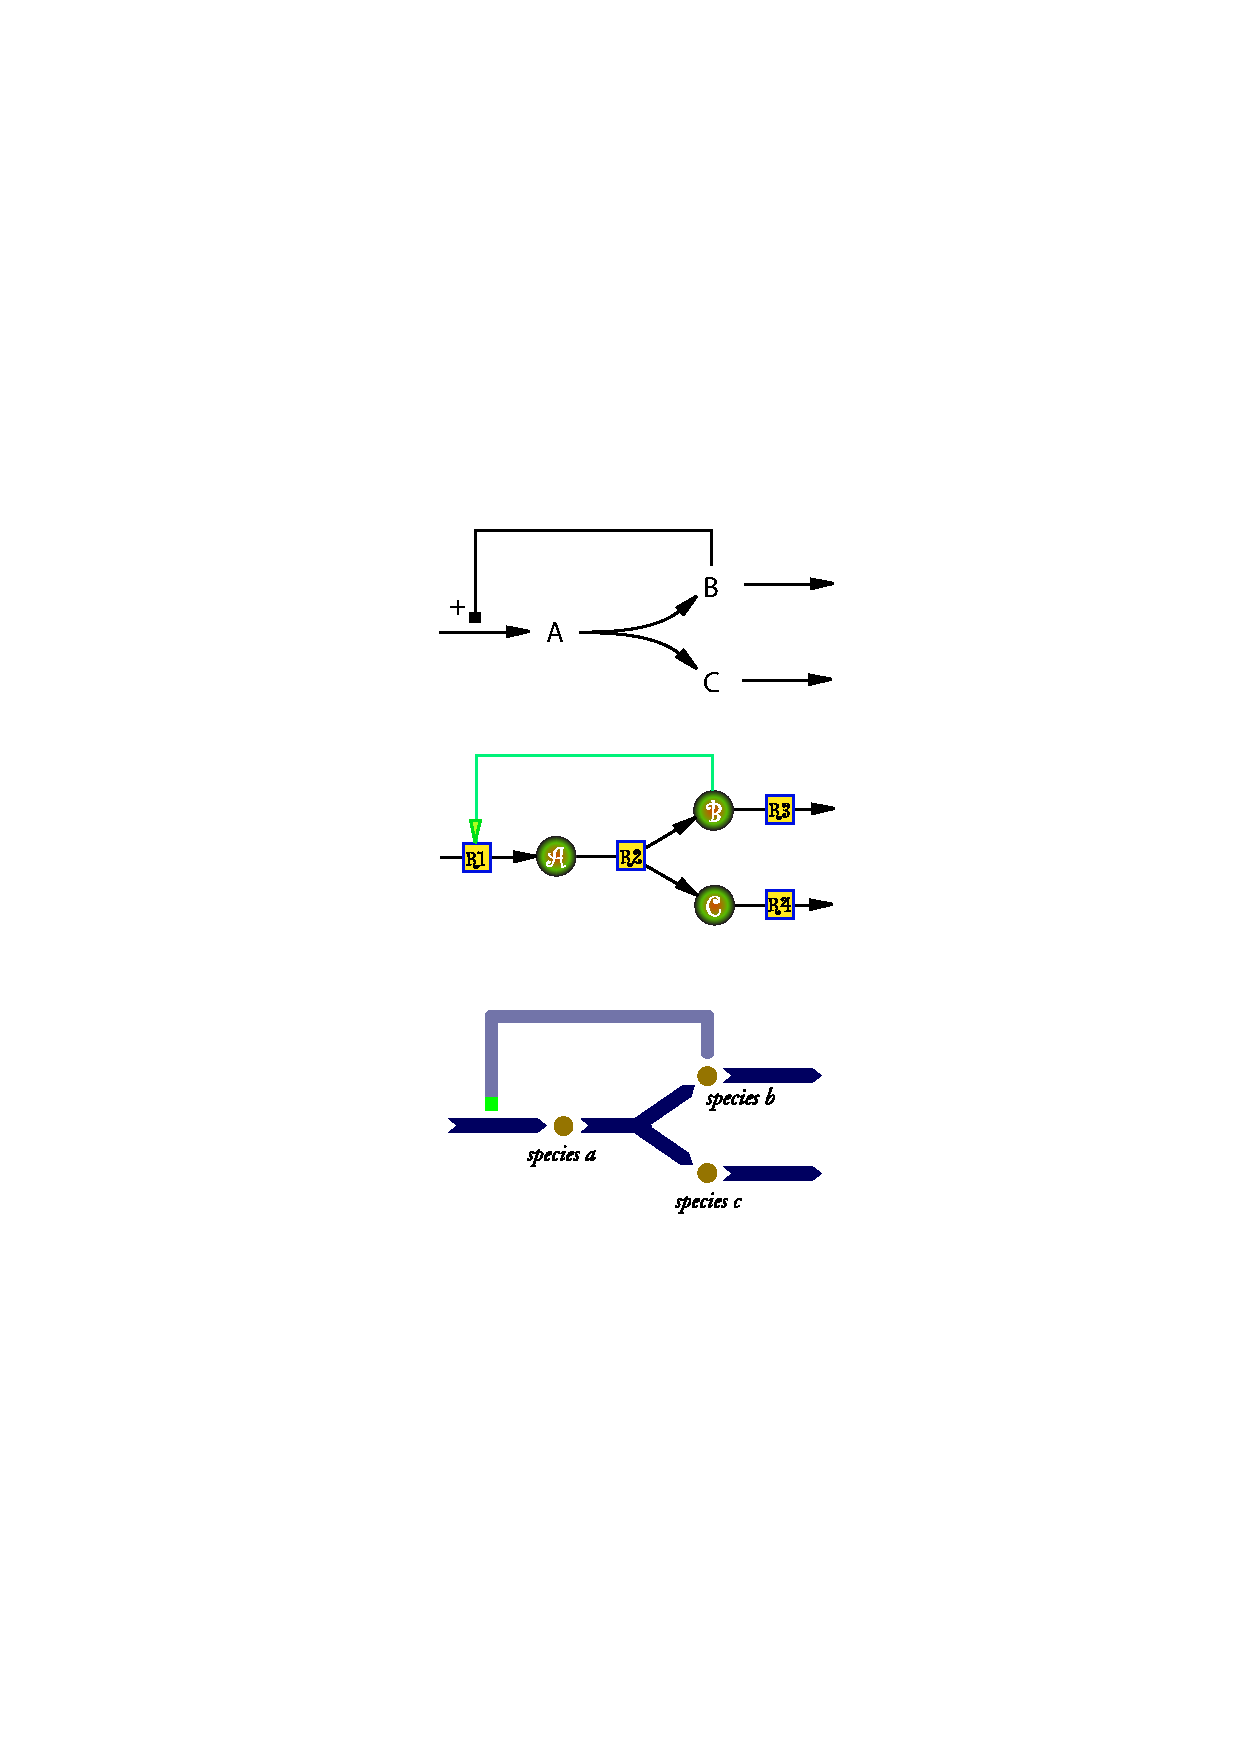
\includegraphics[scale=1]{figures/layout1}
\end{center}
\caption{Illustration of different renderings of the same layout.}
\label{UML:All}
\label{figure:rendering}
\end{figure}
\end{center}

The layout of a reaction network diagram should be described as 
graphical representations of species and reactions (and not as arbitrary 
drawing or graph). This means that existing languages for the 
description of vector drawings (SVG) or general graphs cannot be used. 
While it may seem unnecessary to invent a new language when an existing 
one like SVG could in principle be used to describe the layout of a 
reaction network, there are good reasons to have a language tailored 
specifically for the layout of SBML models. 

Presumably, most programs that will use this SBML extension are 
primarily programs dealing with biochemical models. Internally, they 
will have data structures for species and reactions, so it will be 
natural for them to describe the layout of the reaction network also in 
terms of species and reactions (and not in terms of polygons or 
splines). Thus the \token{layout} object has a similar structure like 
the SBML \token{model} object and contains lists of graphical 
representations of compartments, species, and reactions (called 
\token{compartmentGlyph, speciesGlyph,} and \token{reactionGlyph} 
respectively). Additional layout elements and relationships can be 
represented by using the \token{graphicalObject} and 
\token{generalGlyph} elements. 

Another important question is the level of detail that the description 
should provide. For simplicity, only the layout (i.e., the position of 
the different graphical objects) of the diagram is encoded, not the 
details of how it should be rendered. That is left to the SBML Level~3 
Render package. 

\ref{figure:rendering} illustrates this distinction. All three diagrams 
could be renderings of the same layout and would be described by 
identical SBML files. No information about colors, line styles, fonts, 
etc., is present in the layout description. 

The next question is how the relation between the model and the layout 
should be established. There seems to be consensus that one model 
element can be represented by several layout elements. For example, it 
can be useful to have several representations of one species in the 
layout to avoid crossing lines. This can be accomplished if every layout 
element has a field that refers to the id of a model element. 

There are also cases where a layout element does not correspondent to 
exactly one model element. One example would be if a layout shows a 
simplified version of the model where one reaction in the layout 
corresponds to several reactions and intermediate species in the model. 
This is the reason why the field in the layout elements that refers to 
the model elements is optional, allowing layout objects that do not have 
a specific counterpart in the SBML model. 

The result of all this is a way to describe a graphical layout of a 
reaction network in biochemical terms. This layout can be closely tied 
to the biochemical model. A graphical model editor for example would 
typically create a layout that is closely connected (by a one-to-several 
relation from the model elements to the layout elements) to the model. 

A more general layout design program could also create a layout that is 
not so closely tied to the model, for example, it could create a layout 
that shows a simplified version of the model. 


% -*- TeX-master: "main" -*-

\section{Package syntax and semantics}
\label{sec:syntax}
This section contains a definition of the syntax and semantics of the Spatial package for \sbmlthreecore.  The Spatial package involves several new object classes, and extends the existing \Model, \Compartment, \Species, \Reaction, and \Parameter object class.  \sec{examples} contains complete examples of using the constructs in SBML models.

{\color{red} Lucian: \notice Periodically when I have comments, I'll put them in sections that look like this--in red, with the pointy-hand icon off to the side.  They tend to be design questions I had when creating this document for parts I thought were not clear, or are suggestions for changes that could be made.}


\subsection{Overview of spatial extension}
The SBML \Compartment, \Reaction and \Species, and molecular transport mechanisms (\DiffusionCoefficient, \AdvectionCoefficient, \BoundaryCondition) are mapped to geometric domains to describe spatial models within SBML.  The primary mechanism to accomplish this mapping is to simply map \Compartments to collections of geometric Domains called \DomainTypes.  Each \Domain is a contiguous patch of volumetric space or a contiguous surface patch that is ultimately described by a single system of equations (whichever mathematical framework is used).  In analogy with initial conditions, the mathematical system defined within a domain often needs a definition of what happens at the domain boundary (e.g. boundary conditions) to complete the specification.  Because of this, the boundaries between adjacent domains need to be identified so that appropriate boundary conditions can be specified.  For compactness of representation, rather than map to each individual \Domain, \Compartments are mapped to \DomainTypes, along with the corresponding \Species and \Reactions (with the new compartment attribute).

\subsubsection{Geometry}
The \Geometry object within a model is completely modular and does not reference the rest of the model, promoting reuse of the same geometry in different models.  The geometry separately defines a coordinate system, a list of domain types, a list of domains and their adjacency relationships, and a list of alternate geometric representations.

\subsubsection{Alternative \GeometryDefinitions}
Modeling and simulation tools will each natively support some subset (often just one) of the possible \GeometryDefinitions (analytic, sampled field, constructive solid geometry, and parametric shapes ).  Interoperability will be enhanced if tools write as many geometry definitions as they are able.  Upon reading the model, a tool will typically choose the most convenient geometry definition, i.e. the one that it natively supports.  If a tool does not edit the geometry, it has the ability to preserve the alternate representations during model editing (because the mapping of the model to the geometry is not stored in the geometry).

There are two general classes of geometric representation specification: those that explicitly specify surfaces and those that implicitly specify surfaces.  For example, a level set is a field where a specific isosurface of the field specifies a geometric surface.  A geometry described using constructive solid geometry of geometric primitives (e.g. spheres, cylinders) specifies directly which points are "inside" an object.  Alternatively, explicit surface representations explicitly declare the set of points belonging to surfaces (e.g. polygonal tessellations).



% --------------------------------------------------------------------------
\subsection{Namespace URI and other declarations necessary for using this package}
\label{xml-namespace}
Every SBML Level~3 package is identified uniquely by an XML namespace URI.  For an SBML document to be able to use a given Level~3 package, it must declare the use of that package by referencing its URI.  The following is the namespace URI for this version of the Spatial package for \sbmlthreecore:
\begin{center}
\uri{http://www.sbml.org/sbml/level3/version1/spatial/version1}
\end{center}

In addition, SBML documents using a given package must indicate whether the package can be used to change the mathematical interpretation of a model.  This is done using the attribute \token{required} on the \token{<sbml>} element in the SBML document.  For the Spatial package, the value of this attribute must be \val{true}, because the use of the Spatial package can change the mathematical meaning of a model.

The following fragment illustrates the beginning of a typical SBML model using \sbmlthreecore and this version of the Spatial package:

\begin{example}
<?xml version="1.0" encoding="UTF-8"?>
<sbml xmlns="http://www.sbml.org/sbml/level3/version1/core" level="3" version="1"
      xmlns:spatial="http://www.sbml.org/sbml/level3/version1/spatial/version1"
      spatial:required="true">
\end{example}


\subsection{Primitive data types}
\label{new-primitive-types}

The Spatial package uses a number of the primitive data types described in Section~3.1 of the \sbmlthreecore specification, and adds several additional primitive types described below.


\subsubsection{Type \fixttspace\primtypeNC{SpId}}
\label{primtype-spid}

The type \primtype{SpId} is derived from \primtype{SId}
(\sbmlthreecore specification Section~3.1.7) and has identical syntax. The \primtype{SpId} type is used as the data type for the identifiers of various objects in the Spatial Processes package.  The purpose of having a separate type for such identifiers is to enable the space of possible spatial identifier values to be separated from the space of all other identifier values in SBML.  The equality of \primtype{SpId} values is determined by an exact character sequence match; i.e., comparisons of these identifiers must be performed in a case-sensitive manner.


\subsubsection{Type \fixttspace\primtypeNC{SpIdRef}}
\label{primtype-spidref}

Type \primtype{SpIdRef} is used for all attributes that refer to identifiers of type \primtype{SpId}.  This type is derived from \primtype{SpId}, but with the restriction that the value of an attribute having type \primtype{SpIdRef} must match the value of a \primtype{SpId} attribute in the relevant model;  in other words, the value of the attribute must be an existing spatial identifier in the referenced model.  As with \primtype{SpId}, the equality of \primtype{SpIdRef} values is determined by exact character sequence match; i.e., comparisons of these identifiers must be performed in a case-sensitive manner.


\subsubsection{Type \fixttspace\primtypeNC{BoundaryConditionKind}}
\label{primtype-boundaryconditionkind}

The \primtype{BoundaryConditionKind} primitive data type is used in the definition of the \BoundaryCondition class.  The type \primtype{BoundaryConditionKind} is derived from type \primtype{string} and its values are restricted to being one of the following possibilities: \val{Robin\_valueCoefficient}, \val{Robin\_inwardNormalGradientCoefficient}, \val{Robin\_sum}, \val{\changed{Neumann}}, and \val{\changed{Dirichlet}}.  Attributes of type \primtype{BoundaryConditionKind} cannot take on any other values.  The meaning of these values is discussed in the context of the \BoundaryCondition class's definition in \sec{BoundaryCondition-class}.


\subsubsection{Type \fixttspace\primtypeNC{\changed{CoordinateKind}}}
\label{primtype-componentkind}

The \primtype{\changed{CoordinateKind}} primitive data type is used in the definition of the \CoordinateComponent class.  \primtype{\changed{CoordinateKind}} is derived from type \primtype{string} and its values are restricted to being one of the following possibilities: \val{cartesianX}, \val{cartesianY}, and \val{cartesianZ}.
%, \val{spherical\-Radius}, \val{sphericalAzimuth}, \val{sphericalElevation}, \val{cylindrical\-Radius}, \val{cylindricalAzimuth}, \val{cylindricalHeight}, \val{polarRadius}, and \val{polarAzimuth}.
Attributes of type \primtype{\changed{CoordinateKind}} cannot take on any other values.  The meaning of these values is discussed in the context of the \CoordinateComponent class's definition in \sec{CoordinateComponent-class}.

Other \primtype{\changed{CoordinateKind}} types are held in reserve for future versions of this specification, and may include \val{spherical\-Radius}, \val{sphericalAzimuth}, \val{sphericalElevation}, \val{cylindrical\-Radius}, \val{cylindricalAzimuth}, \val{cylin\-dricalHeight}, \val{polarRadius}, and \val{polarAzimuth}.



%\subsubsection{Type \fixttspace\primtypeNC{CoordinateKind}}
%\label{primtype-coordinatekind}
%
%The \primtype{CoordinateKind} primitive data type is used in the definition of the \CoordinateComponent class.  The type \primtype{CoordinateKind} is derived from type \primtype{string} and its values are restricted to being one of the following possibilities: \val{normal}, \val{symmetrical}, and \val{fixed}.  Attributes of type \primtype{CoordinateKind} cannot take on any other values.  The meaning of these values is discussed in the context of the \CoordinateComponent class's definition in \sec{CoordinateComponent-class}.


\subsubsection{Type \fixttspace\primtypeNC{DiffusionKind}}
\label{primtype-diffusionkind}

The \primtype{DiffusionKind} primitive data type is used in the definition of the \DiffusionCoefficient class.  \primtype{DiffusionKind} is derived from type \primtype{string} and its values are restricted to being one of the following possibilities: \val{isotropic}, \changed{\val{anisotropic}}, and \val{tensor}.  Attributes of type \primtype{DiffusionKind} cannot take on any other values.  The meaning of these two values is discussed in the context of the \DiffusionCoefficient class's definition in \sec{DiffusionCoefficient-class}.


\subsubsection{Type \fixttspace\primtypeNC{FunctionKind}}
\label{primtype-functionkind}

The \primtype{FunctionKind} primitive data type is used in the definition of the \AnalyticVolume class.  The type \primtype{FunctionKind} is derived from type \primtype{string} and its values are restricted to being one of the \changed{single} possibility \val{layered}.  Attributes of type \primtype{FunctionKind} cannot take on any other values.  The meaning of these values is discussed in the context of the \AnalyticVolume class's definition in \sec{AnalyticVolume-class}.


\subsubsection{Type \fixttspace\primtypeNC{GeometryKind}}
\label{primtype-geometrykind}

The \primtype{GeometryKind} primitive data type is used in the definition of the \Geometry class.  \primtype{GeometryKind} is derived from type \primtype{string} and its values are restricted to being the single possibility \val{cartesian}.  Other \primtype{GeometryKind} types are held in reserve for future versions of this specification, and may include \val{cylindrical}, \val{spherical}, and \val{polar}.  Attributes of type \primtype{GeometryKind} cannot take on any other values.  The meaning of these values is discussed in the context of the \Geometry class's definition in \sec{Geometry-class}.


\subsubsection{Type \fixttspace\primtypeNC{SetOperation}}
\label{primtype-setoperation}

The \primtype{SetOperation} primitive data type is used in the definition of the \CSGSetOperator class.  The type \primtype{SetOperation} is derived from type \primtype{string} and its values are restricted to being one of the following possibilities: \val{union}, \val{intersection}, and \val{difference}.  Attributes of type \primtype{SetOperation} cannot take on any other values.  The meaning of these values is discussed in the context of the \CSGSetOperator class's definition in \sec{CSGSetOperator-class}.


\subsubsection{Type \fixttspace\primtypeNC{doubleArray}}
\label{primtype-doublearray}

The \primtype{doubleArray} primitive data type is a space-delimited list of \primtype{double} values in a single string.  


\subsubsection{Type \fixttspace\primtypeNC{integerArray}}
\label{primtype-integerarray}

The \primtype{integerArray} primitive data type is a space-delimited list of \primtype{integer} values in a single string.  

\clearpage


\subsection{The extended \Model object}
\label{extended-model-class}
The \Model object is extended in the spatial package to contain a new \Geometry child, as seen in
\fig{model-uml}. The \Geometry element is contained in the Model element in the 'spatial' namespace. In order to specify a spatial geometry, some of the existing SBML elements need to be extended (\Compartment, \Species, \Parameter, and \Reaction). These extensions to the SBML elements are discussed in the sections that follow.
 
\begin{figure}[ht]
  \includegraphics{figs/extended-model-uml}
  \caption{The definition of the extended \Model object from the Spatial package.  The \Geometry object and its children are defined in their own sections.}
  \label{model-uml}
\end{figure}




\subsection{The extended \Compartment object}
\label{extended-compartment-class}

The \Compartment in the SBML core is extended while defining a spatial model. An SBML model with spatial geometry defines domain types (classes of domains that are anatomically and physiologically similar). These domain types need to be mapped to a compartment in the SBML model. \Compartments are extended to define \CompartmentMappings that map compartments to \DomainTypes such that each corresponding \DomainType is assigned the same biological and mathematical function. Within SBML L3 Core, the compartment Sid refers to the size of that compartment and is specified by the size attribute or may be set by a rule.  For spatial models, the compartment size is calculated as the product of the unit size specified in the compartment mapping and the size of the current domain. The definition for the extension of the Compartment element is shown in \fig{compartment-uml}.
 
\begin{figure}[ht]
  \includegraphics{figs/extended-compartment-uml}
  \caption{The definition of the extension to the \Compartment element, and the definition of the \CompartmentMapping class. The SBML core attributes of \Compartment are not displayed.}
  \label{compartment-uml}
  \label{CompartmentMapping-uml}
\end{figure}



The \Compartment element has an optional \CompartmentMapping child which indicates the \DomainType to which the \Compartment is mapped.  If there is no \CompartmentMapping for a \Compartment in a spatial model, then that \Compartment is excluded from the spatial version of the model.  In the same way, if a \DomainType is not mapped to one or more \Compartments, then the corresponding \Domains in the geometry have no assigned function.


\subsection{The \class{CompartmentMapping} class}
\label{CompartmentMapping-class}
Each \Compartment in a model that defines a spatial geometry may contain an optional \CompartmentMapping. A \CompartmentMapping is defined as part of the model rather than part of the geometry so that the geometry is modular and may be readily shared between models and reused.  A \CompartmentMapping maps a \Compartment defined in the model to a \DomainType defined in the geometry such that each corresponding \DomainType is assigned the same biological and mathematical function described by the set of \Compartments that are mapped to that \DomainType. 

This mapping need not be one-to-one.  In fact, it is common to map er-lumen, er-membrane, and cytosol to the same cell interior volume or 3D \DomainType.  The \token{unitSize} attribute specifies the relative quantity of each \Compartment that is mapped to the \DomainType.

\subsubsection{The \token{\changed{id}} attribute}
The \token{\changed{id}} attribute is a mandatory attribute of type \primtype{SpId} that is used to uniquely identify a \CompartmentMapping in the model.  All identifiers of type \primtype{SpId} must be unique within the \Geometry.  The mathematical value of a \CompartmentMapping is its \token{unitSize} attribute, and can be bound to a \Parameter by using a \SpatialSymbolReference.

\subsubsection{The \token{domainType} attribute}
The mandatory \token{domainType} attribute is of type \primtype{SpIdRef} that indicates a \DomainType defined in the \Geometry element.

\subsubsection{The \token{unitSize} attribute}
The \token{unitSize} attribute is of type \primtype{double} and represents the relative size of the \Compartment with respect to the size of the \Domains to which they are mapped.  Thus for any infinitesimal subset of the \Domain with size S, there exists an amount of Compartment$_{\text{i}}$ of size (S*unitSize$_{\text{i}}$) for i=1..N compartments mapped to that \DomainType.  For example, a 3D \Compartment (and \DomainType) which is mapped to a 3D \DomainType has a \token{unitSize} which is a volume fraction of dimensionless unit.  The total set of all such volume fractions mapped to a particular \DomainType will typically sum to one. 

If the \token{spatialDimensions} attribute of the parent \Compartment is different than the \token{spatialDimension} attribute of referenced \DomainType, the \token{unitSize} attribute is a conversion factor between the two.  The most common example of this would be a 2D \Compartment being mapped to a 3D \DomainType, such as an ER-membrane being mapped to a volumetric cell interior.  In this case, the \token{unitSize} is a surface-to-volume ratio.

If connected to a \Parameter via a \SpatialSymbolReference, an \InitialAssignment may override the value of the \token{unitSize} attribute.  It is theoretically possible to have this value change in time through the use of a \Rule or \Event, but some (if not all) software tools may not support this setup.  If the value is set to change, and the dimensionality of the parent \Compartment and referenced \DomainType is the same, the other \CompartmentMapping elements for the same \DomainType will typically change in concert, so that they continue to sum to one.

Any bound \Parameter's units should be equivalent to the units of the parent \Compartment divided by the units of the referenced \DomainType. 



\subsection{The extended \Species object}
\label{extended-species-class}
The SBML core \Species is extended when a spatial geometry is defined in the model with the addition of a single new required boolean \val{isSpatial} attribute.  The extension to the \Species element is shown in \fig{species-uml}.
 
\begin{figure}[ht]
  \includegraphics{figs/extended-species-uml}
  \caption{The extension to the \Species element. The attributes of \Species from \sbmlthreecore are not displayed.}
  \label{species-uml}
\end{figure}



\subsubsection{The \token{isSpatial} attribute}
The \token{isSpatial} attribute is of data type boolean. If it is set to true, the \Species is spatially distributed in a possibly nonhomogeneous manner within the \Domains of the same type as the mapped \DomainType. 

For continuous deterministic models (described by partial differential equations), a spatial \Species will result in a concentration field described by a partial differential equation which incorporates contributions from \Reactions, diffusion (\DiffusionCoefficient) and advection (\AdvectionCoefficient) and are subject to boundary conditions (\BoundaryCondition) and initial conditions (\InitialAssignment and \Rule).  All of these quantities can be explicit functions of the spatial coordinates as well as spatial and nonspatial \Parameters and \Species.  

For stochastic models, the \Species is represented as a collection of particles that are distributed throughout the \Domains and are subject to reactions, diffusion and advection.  Simulation algorithms either track individual particles (e.g. Particle-based methods) or use spatial discretization to track a large number of well stirred pools (e.g. Next-Subvolume Method).

The \token{compartment} of any \Species set \token{isSpatial} = \val{true} must have a child \CompartmentMapping: if it did not, its compartment would not actually be a part of the spatial model.


\subsection{The extended \Parameter object}
\label{extended-parameter-class}
When an SBML model defines a spatial geometry, the SBML core \Parameter is used to define the diffusion coefficient, transport velocity (advection) and boundary conditions for species and the coordinate components defined in the \Geometry. One \Parameter is created for each quantity, by adding a child \DiffusionCoefficient, \AdvectionCoefficient, or \BoundaryCondition.  Conversely, some elements defined in the spatial package may need to be referenced by mathematics in core constructs, or even have their value set by core constructs such as \InitialAssignment or \Rule.  These spatial elements can be semantically linked to a \Parameter by giving it a child \SpatialSymbolReference pointing to that element.

A \Parameter that has been extended for the Spatial package can have only one of the above listed objects.  For example, if a \Parameter is extended to represent the diffusion coefficient of a species, the existing attributes of the \Parameter (id, name, value, units, constant) are defined according to SBML core specifications, along with a \DiffusionCoefficient child that contains the information about the species it represents. \fig{parameter-uml} represents the extension to the \Parameter element.

\begin{figure}[ht]
  \includegraphics{figs/extended-parameter-uml}
  \caption{The \Parameter element extension for spatial package. The \sbmlthreecore attributes for \Parameter are not displayed in this figure.}
  \label{parameter-uml}
\end{figure}



\subsection{The \class{SpatialSymbolReference} class}
\label{SpatialSymbolReference-class}
A \Parameter is extended with a \SpatialSymbolReference element, when a symbol from the defined spatial geometry (\token{\changed{id}} of any element contained in \Geometry) is required to be used in the SBML core model. Typically, the \SpatialSymbolReference is used to represent the coordinate components defined in the \Geometry's listOfCoordinateComponents.  For example, if the \Geometry is defined in a 2-dimensional Cartesian coordinate system with X and Y defined as coordinate components, two \Parameters (one each for \CoordinateComponents X and Y) are created in the model. The value of the parameter is not required to be set. For each of these parameters, a \SpatialSymbolReference object is created.

\subsubsection{The \token{spatialRef} attribute}
The \token{spatialRef} attribute of \SpatialSymbolReference, is of type \primtype{SpIdRef} and refers to the \changed{\primtype{SpId}} of any element defined in the \Geometry of the model.

\subsection{The \class{DiffusionCoefficient} class}
\label{DiffusionCoefficient-class}
When a species in a spatial model has a diffusion rate constant, a \Parameter for this diffusion constant is created in the SBML model with a \DiffusionCoefficient child, which is used to identify the \Species whose diffusion rate the \Parameter represents. The diffusion coefficient can then be set like any other variable:  its initial value can be set using the \Parameter's \token{value} attribute or through an \InitialAssignment, and if the diffusion coefficient changes in time, this can be defined with a \Rule or \Event. If set, the units of this \Parameter should be length$^2$/time.  If left unset, the \DiffusionCoefficient will inherit the model units of length$^2$/time (typically cm$^2$s$^{-1}$ or um$^2$s$^{-1}$).


It is possible to define both diffusion and advection for the same \Species.

\subsubsection{The \token{variable} attribute}
The required \token{variable} attribute of \DiffusionCoefficient is of type \primtype{SIdRef} and is the \primtype{SId} of the \Species or \Parameter in the model whose diffusion coefficient is being set.

\subsubsection{The \token{type} attribute}
The required \token{type} attribute of \DiffusionCoefficient is of type \primtype{DiffusionKind} and indicates whether the diffusion coefficient is \val{isotropic} (i.e. applies equally in all dimensions/directions) \val{tensor} (i.e. applies only for a particular pair of coordinates), \changed{or \val{anisotropic} (i.e. applies only for a single coordinate)}.  Coefficients of type \val{isotropic} may not have any child \changed{\CoordinateReference} children; coefficients of type \val{tensor} must have exactly two; \changed{and coefficients of type \val{anisotropic} must have exactly one}.


\subsubsection{The \class{\changed{CoordinateReference}} class}
\label{CoordinateReference-class}
The optional \changed{\CoordinateReference} children of the \DiffusionCoefficient object contain \changed{(in their own \token{coordinate} attribute)} the \changed{type} attributes of the \CoordinateComponent (e.g. \changed{\val{cartesianX}, \val{cartesianY}, or \val{cartesianZ}}), for specifying axis or axes it applies to.

\begin{blockChanged}
If the \DiffusionCoefficient has two \CoordinateReference children, the diffusion coefficient is defined for flux in the plane defined by the two \changed{\CoordinateReference} axes.  The diffusion is defined in relation to the direction due to a gradient in the diagonal term of the diffusion tensor for the two coordinates.

If the \DiffusionCoefficient has exactly one \CoordinateReference child, the diffusion is considered to be anisotropic. To be complete, one \DiffusionCoefficient will need to be defined per axis.

If the \DiffusionCoefficient has no \CoordinateReference children, the diffusion is considered to be Isotropic.
\end{blockChanged}

{\color{red} Lucian: \notice Updated again, but still potentially in flux.  We probably need more text here in general to describe the situation.}

\subsubsection{\DiffusionCoefficient uniqueness}
Only one \DiffusionCoefficient may be defined per \Species per pair of valid axes in the \Compartment in which it resides.  Since isotropic diffusion is defined for all axes at once, this means that if an isotropic \DiffusionCoefficient is defined for a \Species, it may have no other diffusuion coefficients.


\subsection{The \class{AdvectionCoefficient} class}
\label{AdvectionCoefficient-class}
The \AdvectionCoefficient is the extension to \Parameter in SBML core that is used to represent transport velocity of a species, if it exists. The transport velocity for the species is defined in a manner similar to the diffusion constant with a unit of length/time (regardless of the units of the corresponding \Species' \val{compartment} attribute).  A \Parameter is created in SBML code for the velocity with an \AdvectionCoefficient child to identify the \Species whose velocity is represented by the \Parameter; its initial value is set either through the \token{value} attribute or an \InitialAssignment.    If the advection coefficient changes in time or space, this can be modeled with a \Rule or \Event.

If defined, the units of the parent \Parameter should be in length/time; if not defined, it inherits from the model-wide units of length divided by the model-wide units of time.

It is possible to define both diffusion and advection for the same \Species.

\subsubsection{The \token{variable} attribute}
The \token{variable} attribute of \AdvectionCoefficient is of type \primtype{SIdRef} and is the SId of the \Species or \Parameter in the model whose advection coefficient (transport velocity) is being set.

\subsubsection{The \token{\changed{coordinate}} attribute}
The \token{\changed{coordinate}} is of type \changed{\primtype{CoordinateKind}} and represents the coordinate component of the velocity. For example, if the \Geometry is defined in the Cartesian coordinate system and is 2-dimensional, the species can have velocity terms for both X and Y. If the \Parameter represents the transport velocity of the species in the X-coordinate, the \token{\changed{coordinate}} attribute will take a value of \changed{\val{cartesianX}}, and if it represents the velocity in the Y-coordinate, the attribute will take a value of \changed{\val{cartesianY}}.  Only one \AdvectionCoefficient may be defined per \Species per valid \token{\changed{coordinate}}.

{\color{red} Lucian: \notice Changed to CoordinateKind.}


\subsection{The \class{BoundaryCondition} class}
\label{BoundaryCondition-class}
A \Species in a spatial model that has a diffusion rate or an advection velocity needs to have specified boundary conditions. A boundary condition is either the concentration of the species or the flux density of the species at a boundary.  The boundary refers to either an internal membrane boundary or a face of the box defined by the minimum and maximum coordinates of the geometry (the geometries bounding box).  

When creating a spatial SBML model, species boundary conditions are created as parameters, one for each boundary condition, by adding a child \BoundaryCondition that points to the corresponding \Species and boundary, depending on the coordinate system.


For Cartesian Geometries, there are two boundaries for every axis being modeled.  For example, in a 2D cartesian geometry for the external boundaries, there could be up to four parameters or parameter sets created for each spatial \Species whose \Compartments abut the minimum and maximums of the X and Y axes).

%For polar and cylendrical Geometries, there is one boundary for the maximum of the radius, and another boundary for the minimum of the radius if that minimum is not \val{0}.  For the azimuth, there are either two boundaries corresponding to the minimum and maximum azimuth, or no boundaries, if the minimum is 0$^\circ$, and the maximum is 360$^\circ$.  In cylendrical geometry, there will be two boundaries for the minumum and maximum height.

%For spherical Geometries, there will again be one boundary for the maximum of the radius, and another boundary for the minumum of the radius if that minimum is not \val{0}.  For the spherical azimuth and elevation, there will be either two boundaries each corresponding to the minimum and maximum values, or no boundaries, for each minimum 0$^\circ$ and maximum 360$^\circ$ pair.

The \Parameter's value is set either through the \token{value} attribute or an \InitialAssignment.  If the boundary condition changes in time, it can be set with a \Rule or \Event.  If set, the \Parameter unit must be equal to the appropriate unit for its \token{type} (see below).  Only one \BoundaryCondition may be defined per \Species per boundary (regardless of type).


\subsubsection{The \token{variable} attribute}
The \token{variable} attribute of \BoundaryCondition is of type \primtype{SIdRef} and is the SId of the \Species or \Parameter in the model whose boundary condition is being set.

\subsubsection{The \token{type} attribute}
The \token{type} attribute is of type \primtype{BoundaryConditionKind} and indicates the type of boundary condition. The boundary condition types come in three groups: for Neumann boundaries, \changed{\val{Neumann} (the inward normal flux)} is used.  For Dirichlet boundaries, \changed{\val{Dirichlet} (the value)} is used.  For Robin boundaries, three different Parameters must be defined, with \BoundaryCondition elements of type \val{Robin\_valueCoefficient}, \val{Robin\_inwardNormalGradientCoefficient}, and \val{Robin\_sum}.

The unit of the boundary condition is determined by the type, and the unit for density and velocity.  For \val{\changed{Dirichlet}}, the unit would be the unit of concentration.  For \val{\changed{Neumann}}, the unit would be concentration*length/time.  For Robin boundaries, for a variable \val{u} with an inward pointing normal vector \val{n}, Robin value coefficient \val{a}, Robin inward normal gradient coefficient \val{b}, and Robin sum \val{g}, the condition is defined by the equation \val{a*u + b*inner\_product(grad(u),n) = g}, with appropriate units.

{\color{red} Lucian: \notice Does this explanation work?}

\subsubsection{The \token{coordinateBoundary} attribute}
The \token{coordinateBoundary} attribute is of type \primtype{SpIdRef} and refers to the \changed{\primtype{SpId}} of either the \token{boundaryMin} or \token{boundaryMax} object of the \CoordinateComponent defined in \Geometry. This \changed{\primtype{SpId}} indicates the boundary condition (minimum or maximum) in the \CoordinateComponent. A \Parameter that is extended with a \BoundaryCondition object can only define the \token{coordinateBoundary} attribute or the \token{boundaryDomainType} attribute, but not both.

\subsubsection{The \token{boundaryDomainType} attribute}
The \token{boundaryDomainType} attribute is of type \primtype{SpIdRef} and refers to the \changed{\primtype{SpId}} of the \DomainType of the location of the species whose boundary condition is being defined. A \Parameter that is extended with a \BoundaryCondition object can only define the \token{coordinateBoundary} attribute or the \token{boundaryDomainType} attribute, but not both. 


\subsection{The extended \Reaction object}
\label{extended-reaction-class}
The SBML core \Reaction is extended when a spatial geometry is defined in the model with the addition of a single new required boolean \token{isLocal} attribute. \fig{reaction-uml} displays the definition of the extension of the \Reaction element.
 
\begin{figure}[ht]
  \includegraphics{figs/extended-reaction-uml}
  \caption{The extension to the \Reaction element. The \sbmlthreecore atrributes and children for \Reaction are not displayed in the figure.}
  \label{reaction-uml}
\end{figure}

\subsubsection{The \token{isLocal} attribute}
The \token{isLocal} attribute for a \Reaction is of type \primtype{Boolean}. The attribute is set to true if the reaction is to be considered a local description of the reaction in terms of concentration/time defined at each point in space rather than substance/time over an entire \Compartment or "pool".  Note that this means that the units of the \KineticLaw are different depending on whether the \Reaction is local or not.


\subsection{The \class{Geometry} class}
\label{Geometry-class}
\label{ListOfCoordinateComponents-class}
\label{ListOfDomainTypes-class}
\label{ListOfDomains-class}
\label{ListOfAdjacentDomains-class}
\label{ListOfGeometryDefinitions-class}

A single geometry must be defined within the model if the spatial extension is to be used. \fig{Geometry-uml} shows the definition of the \Geometry element.
 
\begin{figure}[ht]
  \includegraphics{figs/Geometry-uml}
  \caption{The definition of the \Geometry, \ListOfCoordinateComponents, \ListOfDomainTypes, \ListOfDomains, \ListOfAdjacentDomains, and \ListOfGeometryDefinitions classes from the Spatial package.  The various children of the ListOf- classes are defined in their own sections.}
  \label{Geometry-uml}
  \label{ListOfCoordinateComponents-uml}
  \label{ListOfDomainTypes-uml}
  \label{ListOfDomains-uml}
  \label{ListOfAdjacentDomains-uml}
  \label{ListOfGeometryDefinitions-uml}
\end{figure}

\subsubsection{The \token{\changed{id}} attribute}
The \token{\changed{id}} attribute is of type \primtype{SpId}, uniquely identifies the \Geometry element, and is optional.  It has no mathematical meaning.

\subsubsection{The \token{coordinateSystem} attribute}
The \token{coordinateSystem} attribute is a required attribute and is of type \primtype{GeometryKind}. It represents the coordinate system used by the \Geometry.  A value of  \val{cartesian} indicates that the geometry is a cartesian coordinate system, with the coordinate components corresponding to the x, y, and z components of that system (which could be 1-, 2-, or 3-dimensional).  This is the only coordinate system defined in this version of the specification--in the future, if necessary, \val{cylendrical}, \val{spherical}, and \val{polar} may be added as possibilities, along with n-dimensional cartesian modeling, should there be interest in the modeling community to exchange these types of models.

%A value of \val{cylindrical} indicates that the geometry is a three-dimensional cylendrical coordinate system, with coordinate components corresponding to radial distance, azimuth angle, and axial position.  A value of \val{spherical} indicates that the geometry is a three-dimensional spherical coordinate system, with coordinate components corresponding to radial distance, polar angle, and azimuth angle.  A value of \val{polar} indicates that the geometry is a two-dimensional polar coordinate system, with coordinate components corresponding to radial distance and angle (the two-dimensional equivalent of the cylendrical coordinate system).

\subsubsection{The listOf container classes}
The \Geometry has listOfCoordinateComponents, listOfDomainTypes, listOfDomains, and listOfAdjacentDomains, and listOfGeometryDefinitions that help define the geometry.  The \ListOfCoordinateComponents is a list of \CoordinateComponent objects, the \ListOfDomainTypes is a list of \DomainType objects, the \ListOfDomains is a list of \Domain objects, \ListOfAdjacentDomains is a list of \AdjacentDomains objects, and the \ListOfGeometryDefinitions is a list of alternative \GeometryDefinitions (\ParametricGeometry,\CSGeometry, \SampledFieldGeometry, \AnalyticGeometry).  None of these lists are technically required, but, if present, none of them may be empty.

Note that the children of the \ListOfGeometryDefinitions object are not called \token{geometryDefinition} but rather take the name of the derived class, decapitalized.  Thus, they may be called \token{parametricGeometry}, \token{sampledFieldGeometry}, \token{csGeometry}, or \token{analyticGeometry}.


\subsection{The \class{CoordinateComponent} class}
\label{CoordinateComponent-class}
A \CoordinateComponent object explicitly defines a coordinate component of the coordinate axes and gives them names, units, and formally associates them with a coordinate system. The \CoordinateComponent also defines the minimum and maximum values of the coordinate axis it represents. The definition of \CoordinateComponent is shown in \fig{CoordinateComponent-uml}.
 
\begin{figure}[ht]
  \includegraphics{figs/CoordinateComponent-uml}
  \caption{The \CoordinateComponent object definition. One or more instances of \CoordinateComponent objects in a \ListOfCoordinateComponents can be present in \Geometry.}
  \label{CoordinateComponent-uml}
\end{figure}


\subsubsection{The \token{\changed{id}} attribute}
A \CoordinateComponent is identified with the \token{\changed{id}} attribute which is of type \primtype{SpId}.  When referenced (for example, via a \SpatialSymbolReference extension of the SBML core \Parameter object) and used within a mathematical expression, it represents the coordinate value for this \CoordinateComponent.
 
Because a \CoordinateComponent represents an entire axis, it is not appropriate, should it be connected to a \Parameter via a \SpatialSymbolReference, for that \Parameter to be set via an \InitialAssignment or \Rule.  Rather, it is treated like the SBML core \token{csymbol} \val{time}, and can be used as an independent variable in other calculations.

\subsubsection{The \token{\changed{type}} attribute}
The \token{\changed{type}} attibute of type \primtype{\changed{CoordinateKind}} represents the type of the coordinate component, and may take one of a subset of all possible \primtype{\changed{CoordinateKind}} values depending on its parent \Geometry, as defined in \tab{CoordinateComponent-Geometry-relation}.
%For all \primtype{GeometryKind} values except \val{cartesian}, exactly one \CoordinateComponent must exist with each of the allowed \primtype{\changed{CoordinateKind}} values:  in other words, a \val{cylendrical} \Geometry must have exactly three \CoordinateComponent children, each one having a different allowed value for its \token{\changed{type}} attribute.
For Cartesian geometries, one-dimensional geometries may be defined by having a single \val{cartesianX} \CoordinateComponent; two-dimensional geometries may be defined by having two \CoordinateComponent children with \token{\changed{type}} values of \val{cartesianX} and \val{cartesianY}, and three-dimensional geometries may be defined by having three \CoordinateComponent children with \token{\changed{type}} values of \val{cartesianX}, \val{cartesianY}, and \val{cartesianZ}.

\begin{table}[thb]
  \begin{edtable}{tabular}{>{\centering\arraybackslash}m{0.9in} >{\centering\arraybackslash}m{0.7in} >{\raggedright\arraybackslash}m{4.4in}}
  %\begin{edtable}{tabular}{p{0.9in}p{0.7in}p{4.4in}}
    \toprule
    \textbf{GeometryKind} & \textbf{Dimensions} & \textbf{\changed{CoordinateKind}s} \\
    \midrule
    \token{cartesian}   & 1 & \val{cartesianX} (\token{coord1})\\
    \token{cartesian}   & 2 & \val{cartesianX} (\token{coord1}) and \val{cartesianY} (\token{coord2})\\
    \token{cartesian}   & 3 & \val{cartesianX} (\token{coord1}), \val{cartesianY} (\token{coord2}), and \val{cartesianZ} (\token{coord3})\\
 %   \token{cylendrical} & 3 & \val{cylindricalRadius} (\token{coord1}), \val{cylindricalAzimuth} (\token{coord2}), and \val{cylindricalHeight} (\token{coord3})\\
 %   \token{polar}       & 2 & \val{polarRadius} (\token{coord1}) and \val{polarAzimuth} (\token{coord2})\\
 %   \token{spherical}   & 3 & \val{sphericalRadius} (\token{coord1}), \val{sphericalAzimuth} (\token{coord2}), and \val{sphericalElevation} (\token{coord3})\\
    \bottomrule
  \end{edtable}
  \caption{Correspondance between the \token{type} of a \Geometry and the possible \token{\changed{type}}s of its child \CoordinateComponent elements.  Also noted is the corresponding attribute (\token{coord1}, \token{coord2}, or \token{coord3}) corresponding to each axis when defining \InteriorPoint elements (see \sec{InteriorPoint-class}).} 
  \label{CoordinateComponent-Geometry-relation}
\end{table}



%\subsubsection{The \token{coordinateType} attribute}
%The \token{coordinateType} attribute, of type \primtype{CoordinateKind}, represents whether the axis being defined is normal (\val{normal}), or whether it represents a dimension that does not need to be modeled explicitly in any performed calculations, whether due to symmery, where the modeled element exists in the given dimension, but is assumed to be the same for all values along that axis (\val{symmetrical}), or due to being constrained to a single value along that axis (\val{fixed}).

%\CoordinateComponent elements of coordinateType \val{normal} must have a \token{boundaryMin} and \token{boundaryMax} child.  \CoordinateComponent elements of coordinateType \val{symmetrical} may have a \token{boundaryMin} and \token{boundaryMax} children for visualization purposes, but they are optional.  \CoordinateComponent elements of coordinateType \val{fixed} must have a single \token{boundaryFixed} child.

{\color{red} Lucian: \notice coordinateType attribute removed.}


\subsubsection{The \token{unit} attribute}
The unit of a \CoordinateComponent is represented by the \token{unit} attribute, of type \primtype{UnitSIdRef}.  If not specified, the unit of a \CoordinateComponent inherits from the \token{lengthUnits} attribute of the \Model object, and if that in turn is not specified, the \CoordinateComponent units cannot be determined.
%Many coordinates may have different units from the \token{lengthUnits} of the \Model, since this is a distance metric and not always the same as the unit of each individual coordinate.  For example, in Polar coordinates, the coordinate component 'theta' may be described in radians while component 'rho' may be in microns.  


\subsection{The \class{Boundary} class}
\label{Boundary-class}
The minimum and the maximum for a \CoordinateComponent represent the bounds in each coordinate.  For example, for three dimensional Cartesian coordinate system with x, y, and z coordinates, the minimum and maximum limits for each coordinates define planes orthogonal to each coordinate axis and passing through the minimum or maximum.  If max-min is the same for each x,y,z then the bounds on the geometry is a cube.  The \Boundary class interacts with the \BoundaryCondition class, allowing modelers to define how model elements behave at the boundary of the model.  For species defined within volumes adjacent to these surfaces, \BoundaryCondition elements must be introduced.

{\color{red} Lucian: \notice Just a note to coordinate the text here to sync with the text in the \BoundaryCondition class, if that changes.  }

The minimum limit of a \CoordinateComponent is represented by the \token{boundaryMin} object and the maximum limit is represented by the \token{boundaryMax} object, and apply to \CoordinateComponent elements.
%of coordinateType \val{normal} and \val{symmetrical} (and are optional in the latter case only).
Both are \Boundary objects, and have the following attributes:

%For \CoordinateComponent elements of coordinateType \val{fixed}, a single \token{boundaryFixed} object defines the value at which the coordinate component is fixed.  

\subsubsection{The \token{\changed{id}} attribute}
The \token{\changed{id}} attribute of the \Boundary object identifies the object. The attribute is required and is of type \primtype{SpId}. This attribute is used when specifying the \BoundaryCondition for a species as an extension of an SBML core \Parameter.   When referenced (for example, via a \SpatialSymbolReference extension of the SBML core \Parameter object) and used within a mathematical expression, it represents the value of the \Boundary.  The units are the same as its parent \CoordinateComponent, and are not set separately.

\subsubsection{The \token{value} attribute}
The \token{value} attribute is of type \primtype{double}. In a \token{boundaryMin} object, it represents the minimum limit of the \CoordinateComponent.  In a \token{boundaryMax} object, it represents the maximum limit of the \CoordinateComponent.

%In a \token{boundaryFixed} object, it represents the fixed level of the \CoordinateComponent.

If connected to a \Parameter via a \SpatialSymbolReference, this \token{value} may be overridden by an \InitialAssignment.  It is theoretically possible to have this value change in time through the use of a \Rule or \Event, but some (if not all) software tools may not support this setup. 


\subsection{The \class{DomainType} class}
\label{DomainType-class}
A \DomainType is a class of domains that are identified as being anatomically and physiologically similar.  For example, a \DomainType "cytosol" may be defined in a \Geometry as identifying the structure and function of the cell interior.  If there is one cell, then there is one domain, if there are multiple cells, then there are multiple disjoint domains ("cytosol1","cytosol2", etc.) identified with the \DomainType "cytosol".  \CompartmentMappings, defined as an extension to an SBML core \Compartment, map compartments to domain types such that each corresponding domain is assigned the same biological and mathematical function. \fig{DomainType-uml} shows the \DomainType object.

Each SBML \Compartment maps to a single \DomainType, meaning that the initial condition of each \Species in each \Compartment will be the same across all \Domains that map to a given \DomainType.  If those \Species are spatially distributed, they will subsequently evolve independently from each other.  However, if modeling two \Domains that are similar but whose \Species have different initial conditions, those \Domains should be modeled as separate \DomainTypes.

\begin{figure}[ht]
  \includegraphics{figs/DomainType-uml}
  \caption{The \DomainType object. One or more instances of \DomainType in a \ListOfDomainTypes instance can be present in a \Geometry object.}
  \label{DomainType-uml}
\end{figure}

\subsubsection{The \token{\changed{id}} attribute}
Each \DomainType is identified with a \token{\changed{id}} of type \primtype{SpId}.  When referenced and used within a mathematical expression, it represents the sum of the sizes of all domains associated with this \DomainType.

As a derived quantity, if connected to a \Parameter via a \SpatialSymbolReference, this value may \emph{not} be overridden by an \InitialAssignment, nor by the use of a \Rule or \Event.  Its value is always connected to the size of its component \Domains instead.  The units of a \DomainType are the units of the corresponding base units of the SBML \Model for length (for one-dimensional domains), area (for two-dimensional domains), or volume (for three-dimensional domains).  It is required to define the corresponding base units for every \DomainType in the \Model.

\subsubsection{The \token{spatialDimension} attribute}
The \token{spatialDimension} attribute of the \DomainType is of type \primtype{int} and can take on a value of 0, 1, 2, or 3. The spatial dimension is specified for a \DomainType, rather than being repeated for each \Domain that is represented by the \DomainType.

{\color{red} Lucian: \notice The equivalent attribute of a \Compartment is \token{spatialDimensions}, i.e. it has an 's' on the end.  Can we change this to match?}


\subsection{The \class{Domain} class}
\label{Domain-class}
\label{ListOfInteriorPoints-class}
\Domains represent contiguous regions identified by the same \DomainType.  One, two and three dimensional domains are contiguous linear regions, surface regions, and volume regions (respectively), bounded by the limits of the coordinate system (e.g. min/max of x,y,z) and adjacent domains corresponding to different domain types.  \Domain is shown in \fig{Domain-uml}.
 
\begin{figure}[ht]
  \includegraphics{figs/Domain-uml}
  \caption{The definition of the \Domain, \ListOfInteriorPoints, and \InteriorPoint classes.  A \ListOfDomains instance in \Geometry can contain one or more \Domain object instances.}
  \label{Domain-uml}
  \label{InteriorPoint-uml}
  \label{ListOfInteriorPoints-uml}
\end{figure}

\subsubsection{The \token{\changed{id}} attribute}
A \Domain is identified with an \changed{\token{id}} attribute of type \primtype{SpId}.  This \token{\changed{id}} may be used within a \SpatialSymbolReference object that is extended from an SBML core \Parameter and can be used in an expression.  When referenced, the domain evaluates to the absolute size of that domain as used by the simulator (the meshed size).

As a derived quantity, if connected to a \Parameter via a \SpatialSymbolReference, this value may \emph{not} be overridden by an \InitialAssignment, nor by the use of a \Rule or \Event.  Its value is always connected to the size of the corresponding \Geometry instead.  The units of the \Domain are the same as the units of the corresponding \DomainType.

\subsubsection{The \token{domainType} attribute}
The \token{domainTpe} attribute refers to the \changed{\primtype{SpId}} of the \DomainType that describes the anatomy and physiology of this domain. The attribute is of type \primtype{SpIdRef}. It is through this association that compartments, and hence the whole SBML model, gets mapped to the individual domains. 


\subsection{The \class{InteriorPoint} class}
\label{InteriorPoint-class}
Each \Domain can contain a \ListOfInteriorPoints. The list of spatial points for a domain is interior to that domain.  This list is optional for a \Domain if it is the only \Domain defined for its \DomainType, but is required otherwise.

For those geometric descriptions that can describe multiple disjoint domains belonging to the same \token{domainType}, these interior points allow unambiguous identification of each domain.  Formally, a single point would suffice, but in practice some tools (e.g. Smoldyn) require multiple points to handle non-convex volumes bounded by explicit surfaces.  For discontinuous surfaces with the same \token{domainType}, the interior point identifies which domain is associated with which surface patch defined in the geometry definition.

Each \InteriorPoint has three attributes: \token{coord1}, \token{coord2}, and \token{coord3}. 

\subsubsection{The \token{coord1}, \token{coord2}, and \token{coord3} attributes}
An InteriorPoint element represents a single point within the defined coordinate system and should be in the interior of the domain that contains it. It has three attributes, \token{coord1}, \token{coord2}, and \token{coord3}, of type \primtype{double}, representing the position along each of the up to three coordinate axes defined by the \CoordinateComponents \changed{(with \token{type} \val{cartesianX}, \val{cartesianY}, and \val{cartesianZ}, respectively, for each \token{coord\_} attribute}; see \tab{CoordinateComponent-Geometry-relation}).

Each \InteriorPoint must define the same number of attributes as there are dimensions of the corresponding \Geometry to which it belongs.

In the case of surfaces, interior points are sometimes required to make unambiguous identification of multiple surfaces (e.g multiple plasma membranes for multiple cells present in a geometry).  Due to roundoff error and finite word lengths, it is difficult to find a three dimensional point that lies on a surface.  In this case, the distance from the surface will be used to provide unambiguous identification.


\subsection{The \class{AdjacentDomains} class}
\label{AdjacentDomains-class}
\AdjacentDomains (or domain adjacencies) captures the topological relationships within the \Geometry.  Consider that the \Domains are nodes in a graph. The \AdjacentDomains objects are the edges that specify the spatial connectivity of these nodes.  Armed with the topology and the domain sizes, one can readily perform a compartmental approximation.  \fig{AdjacentDomains-uml} shows the definition of the \AdjacentDomains object.

\begin{figure}[ht]
  \includegraphics{figs/AdjacentDomains-uml}
  \caption{The definition of the \AdjacentDomains class. \Geometry can contain one instance of \ListOfAdjacentDomains that can have one or more instances of \AdjacentDomains objects.}
  \label{AdjacentDomains-uml}
\end{figure}

\subsubsection{The \token{\changed{id}} attribute}
This attribute identifies an \AdjacentDomains object. The attribute is of type \primtype{SpId}.  It has no mathematical meaning.

\subsubsection{The \token{domain1} and \token{domain2} attributes}
The \token{domain1} and \token{domain2} attributes, of type \primtype{SpIdRef}, are required attributes. They are the \changed{\primtype{SpId}}'s of two domains that touch each other (spatially adjacent).  These are typically surface-volume contacts.


\subsection{The \class{GeometryDefinition} class}
\label{GeometryDefinition-class}
A \Geometry can specify a list of \GeometryDefinitions. The \GeometryDefinition is an abstract class that is the general term for the container which defines the concrete geometric constructs represented by the \Geometry. Four types of \GeometryDefinitions have been identified - \AnalyticGeometry, \SampledFieldGeometry, \ParametricGeometry, \CSGeometry (Constructed Solid Geometry) - and are elaborated in the following sections. The definition of the \GeometryDefinition element is displayed in \fig{GeometryDefinition-uml}.  The spatial dimension of the \GeometryDefinition must match the \token{spatialDimension} of the \DomainType defined for the associated \Domain.

\begin{figure}[ht]
  \includegraphics{figs/GeometryDefinition-uml}
  \caption{The \GeometryDefinition element. \Geometry contains one instance of listOfGeometryDefinitions that can contain one or more instances of \GeometryDefinition (one of \AnalyticGeometry, \SampledFieldGeometry, \CSGeometry, \ParametricGeometry, defined below).}
  \label{GeometryDefinition-uml}
\end{figure}

\subsubsection{The \token{\changed{id}} attribute}
The \token{\changed{id}} attribute that is common to all the \GeometryDefinition types is used to uniquely identify the \GeometryDefinition. The attribute is of type \primtype{SpId}.  A \GeometryDefinition has no mathematical meaning.


\subsection{The \class{AnalyticGeometry} class}
\label{AnalyticGeometry-class}
\label{ListOfAnalyticVolumes-class}
The \AnalyticGeometry is a class of \GeometryDefinition where the geometry of each domain is defined by an analytic expression. An \AnalyticGeometry is defined as a collection of \AnalyticVolumes, one \AnalyticVolume for each volumetric domain in the geometry. In this representation, the surfaces are treated as the boundaries between dissimilar \AnalyticVolumes. The \AnalyticGeometry object contains a \ListOfAnalyticVolumes. \fig{AnalyticGeometry-uml} shows the definition of the \AnalyticGeometry object.

\begin{figure}[ht]
  \includegraphics{figs/AnalyticGeometry-uml}
  \caption{The definition of the \AnalyticGeometry, \ListOfAnalyticVolumes, and \AnalyticVolume classes.}
  \label{AnalyticGeometry-uml}
  \label{ListOfAnalyticVolumes-uml}
  \label{AnalyticVolume-uml}
\end{figure}


\subsection{The \class{AnalyticVolume} class}
\label{AnalyticVolume-class}
The \AnalyticVolume is used to specify the analytic expression of a volumetric (3-dimensional) domain. The analytic expression for the \AnalyticVolume is defined in the Math element.

\subsubsection{The \token{\changed{id}} attribute}
The \token{\changed{id}} attribute uniquely identifies the \AnalyticVolume. The attribute is required and is of type \primtype{SpId}.  It has no mathematical meaning.

\subsubsection{The \token{functionType} attribute}
The \token{functionType} attribute is of type \primtype{FunctionKind} and is currently limited to just \val{layered} \changed{(a possibility for future versions of the specification is to allow the value \val{R-function})}.  A \val{layered} function type implies that the Math child element contains an inequality in the spatial dimensions (e.g. x,y,z) such that evaluation to \val{true} indicates that the point (x,y,z) is within that shape, and "false" indicates that it is not covered by that shape.
%The \val{R-function} \token{functionType} indicates that the shape is represented by a real-valued function whose sign indicates coverage by the shape.

{\color{red} Lucian: \notice If you want to rename 'layered', now is the time to do it ;-)}

\subsubsection{The \token{domainType} attribute}
The \token{domainType} attribute of type \primtype{SpIdRef} is a required attribute. It represents the \changed{\primtype{SpId}} of the \DomainType of the \Domain that is represented by this \AnalyticVolume. 

\subsubsection{The \token{ordinal} attribute}
The \token{ordinal} attribute of type \primtype{int} is an optional attribute. It is used to represent the order of the \AnalyticVolume. The \token{ordinal} is useful while reconstructing the geometry in the specific software tool - it represents the order in which the \AnalyticVolumes representing geometric domains have to be evaluated.

Rather than struggle with the task of preventing overlapping regions of space from different \AnalyticVolumes, the \AnalyticVolumes are to be considered to be evaluated in the reverse order of their ordinals.  In this way, any \AnalyticVolumes that have already been processed will cover those with a smaller ordinal, thus resolving any ambiguities and removing the constraint that all \AnalyticVolumes be disjoint and cover the entire geometric domain.  The \AnalyticVolume with \token{ordinal} 0 can be the "background" layer (typically the extracellular space).  

No two \AnalyticVolumes may have the same \token{ordinal} value, even if they should not overlap, because some tools may not calculate the geometries to the same level of precision as other tools, and may end up with overlap due to rounding errors, and will still need to resolve the ambiguity for their own purposes.  Any \AnalyticVolume without an \token{ordinal} value should also not overlap with any other \AnalyticVolume, but if it does, the software tool may resolve the situation however it sees fit.


\subsection{The \class{Math} class}
\label{Math-class}
The Math element is a required element for an \AnalyticVolume. The Math element contains a MathML expression that defines the analytic expression for the \AnalyticVolume referencing the coordinate components that are specified in the \ListOfCoordinateComponents in the \Geometry, according to the \token{functionType}. 


\subsection{The \class{SampledFieldGeometry} class}
\label{SampledFieldGeometry-class}
\label{ListOfSampledVolumes-class}
\SampledFieldGeometry is a type of \GeometryDefinition that defines a sampled image-based geometry or a geometry based on samples from a level set. \SampledFieldGeometry is defined using a \SampledField that specifies the sampled image and a list of \SampledVolumes that represent the volumetric domains as sampled image regions. \fig{SampledFieldGeometry-uml} shows the definition of the \SampledFieldGeometry object.  It may be used for geometries of any dimension.

\begin{figure}[ht]
  \includegraphics{figs/SampledFieldGeometry-uml}
  \caption{The definition of the \SampledFieldGeometry, \ListOfSampledVolumes, \SampledVolume, \SampledField, and \ImageData classes.}
  \label{SampledFieldGeometry-uml}
  \label{ListOfSampledVolumes-uml}
  \label{SampledVolume-uml}
  \label{SampledField-uml}
  \label{ImageData-uml}
\end{figure}



\subsection{The \class{SampledVolume} class}
\label{SampledVolume-class}
A \SampledVolume represents an interval of the sampled field that constitutes one or more contiguous regions. A \SampledVolume is defined for each volumetric (3-dimensional) \Domain in the \Geometry. It has the following attributes.

\subsubsection{The \token{\changed{id}} attribute}
The \token{\changed{id}} attribute identifies a \SampledVolume object. The attribute is of type \primtype{SpId} and is required when specifying a \SampledVolume.  It has no mathematical meaning.

\subsubsection{The \token{domainType} attribute}
The required \token{domainType} attribute is of type \primtype{SpIdRef}. It is the \changed{\primtype{SpId}} of the \DomainType that represents this class of anatomical features. If there are more than one contiguous regions, then more than one domain will be defined corresponding to each \SampledVolume.

\subsubsection{The \token{sampledValue} attribute}
The required \token{sampledValue} attribute is of type \primtype{double}. It represents the pixel value of a \SampledVolume.

\subsubsection{The \token{minValue} attribute}
The optional \token{minValue} attribute is of type \primtype{double}. It represents the minimum of the pixel value (\token{sampledValue}) range.

\subsubsection{The \token{maxValue} attribute}
The optional \token{maxValue} attribute is of type \primtype{double}. It represents the maximum of the pixel value (\token{sampledValue}) range.


\subsection{The \class{SampledField} class}
\label{SampledField-class}
A \SampledField defined in a \SampledFieldGeometry is a sampled scalar field such as an image or samples from a level set. Currently, the attributes of \SampledField represent the specification of an image dataset (the number of samples in x, y, z coordinates, data type of the image representation, etc.) and the ImageData element of the \SampledField specifies the actual image as integer sampled data.

\subsubsection{The \token{\changed{id}} attribute}
The \token{\changed{id}} attribute identifies a \SampledField. It is of type \primtype{SpId} and is a required attribute.  It has no mathematical meaning.

\subsubsection{The \token{numSamples1}, \token{numSamples2}, \token{numSamples3} attributes}
The \token{numSamples1}, \token{numSamples2}, and \token{numSamples3} attributes represent the number of samples in each of the coordinate components. (e.g. numX, numY, numZ) in an image dataset.  These attributes are of type \primtype{int} and are required to specify the \SampledField. The samples are assumed to be uniformly sampled.

\subsubsection{The \token{dataType} attribute}
This attribute represents the data type of each sample (e.g. int32). The attribute is of type \primtype{string} and is optional.

{\color{red} Lucian: \notice This attribute seems a bit arbitrary, and unhelpful unless there's a standard list of possible values here.  Is there one?  If not, I say we drop the attribute entirely.}


\subsubsection{The \token{interpolationType} attribute}
The \token{interpolationType} attribute is an optional attribute of type \primtype{string} and represents the interpolation type of the sampled data and is defined as "constant" for zeroth order, "linear" for first order, etc.

{\color{red} Lucian: \notice Again, the list of possible values here needs to be explicitly stated.  If it really can be any arbitrary order, switching this to a non-negative integer would make more sense.}

\subsubsection{The \token{encoding} attribute}
The \token{encoding} attribute is an optional attribute of type \primtype{string}. It is used to specify text encoding and compression.

{\color{red} Lucian: \notice Again, the list of possible values here needs to be explicitly stated, if it makes any difference to the model.  Unless you really want people to be able to put in 'standard zip' or 'rot13' as their encoding type.}


\subsection{The \class{ImageData} class}
\label{ImageData-class}
The ImageData element represents the actual image data of the image-based geometry as encoded samples defined by the encoding and the data type. The ImageData element has the following attributes.

\subsubsection{The \token{samples} attribute}
The \token{samples} attribute is of type \primtype{integerArray}, whose values represent the image pixel values. This attribute is required.

\subsubsection{The \token{samplesLength} attribute}
The \token{samplesLength} attribute is of type \primtype{int} and is required. It represents the array length of the \token{samples} attribute (number of values in the image data array).

\subsubsection{The \token{dataType} attribute}
The \token{dataType} attribute is of type \primtype{string} and is required. Presently, this attribute indicates if the image data is 'compressed' or 'uncompressed'.  {\color{red} Anu: \notice (This attribute and the \token{encoding} attribute of \SampledField have to be revisited.)}

{\color{red} Lucian: \notice I agree!}

\subsection{The \class{CSGeometry} class}
\label{CSGeometry-class}
\label{ListOfCSGObjects-class}
\CSGeometry (Constructed Solid Geometry) is a type of \GeometryDefinition that defines a combined, solid, volumetric object from a number of primitive solid volumes by the application of set operations such as union, intersection and difference and affine transformations such as rotation, scaling, translation, etc. The \CSGeometry element is defined by a \token{listOfCSGObjects} element that contains a collection of \CSGObjects. \fig{CSGeometry-uml} shows the definition of the \CSGeometry object.

\begin{figure}[ht]
  \includegraphics{figs/CSGeometry-uml}
  \caption{The definition of the \CSGeometry, \ListOfCSGObjects, and \CSGObject classes.}
  \label{CSGeometry-uml}
  \label{ListOfCSGObjects-uml}
  \label{CSGObject-uml}
\end{figure}



\subsection{The \class{CSGObject} class}
\label{CSGObject-class}
Each \CSGObject is a scene graph representing a particular geometric object using constructed solid geometry. A node in a tree (scene graph) is made up of \CSGPrimitives, \CSGSetOperators, and \CSGTransformations.  Note that the \CSGPrimitives are always leaves in this tree. The \CSGObject is analogous to an \AnalyticVolume element in the sense that it is a constructed geometry (from primitives) used to specify a volumetric (3-dimensional) domain. The \CSGObject element has three attributes : \token{\changed{id}}, \token{domain} and \token{ordinal}. The definition of the \CSGObject is completed by defining a \CSGNode which is the root of the \CSGObject scene graph.

\subsubsection{The \token{\changed{id}} attribute}
The \token{\changed{id}} attribute uniquely identifies the \CSGObject element. The attribute is required and is of type \primtype{SpId}. 

{\color{red} Lucian: \notice Does this element have mathematical meaning?}

\subsubsection{The \token{domain} attribute}
The \token{domain} attribute is of type \primtype{SpIdRef} and is a required attribute. It is a reference to the \token{\changed{id}} of the \Domain that this \CSGObject represents.

{\color{red} Lucian: \notice Am I correct in assuming that this information is redundant with the corresponding \Domain's interior points list?  Is this information necessarily redundant?  Is that OK?  I'm going to assume that the following is a reasonable restriction:}

All \InteriorPoints of the corresponding \Domain must be points inside the geometry this \CSGObject describes.

\subsubsection{The \token{ordinal} attribute}
The \token{ordinal} attribute of type \primtype{int} is an optional attribute. It is used to represent the order of the \CSGObject. The \token{ordinal} is useful while reconstructing the geometry in the specific software tool - it represents the order in which the \CSGObjects representing geometric domains have to be placed.

{\color{red} Lucian: \notice We should probably be as explicit here as we were with the similar \val{ordinal} attribute of the \AnalyticVolume class.  Can I assume that the same rules apply and copy the text here?  One oddness is that the \val{ordinal} attribute of the \AnalyticVolume class is optional, while here it is required.  If they do the same thing, we should probably either make them both optional, or both required.}


\subsubsection{The [\token{csgNode}] child}

The child [\token{csgNode}] element represents the geometry that is to be linked to the \token{domainType} of the \CSGObject.  Note that the child of the \CSGObject element is not called \val{csgNode} but rather takes the name of the derived class, decapitalized.  Thus, a \CSGObject may have a \token{csgPrimitive}, \token{csgPseudoPrimitive}, \token{csgSetOperator}, \token{csgTranslation}, \token{csgRotation}, \token{csgScale}, or \token{csgHomogeneousTransformation} child.


\subsection{The \class{CSGNode} class}
\label{CSGNode-class}
The operators and operands used to construct a constructed solid geometry are generalized as a \CSGNode, defined in \fig{CSGNode-uml} as an abstract base class. The classes that inherit from \CSGNode can be one of the following: \CSGSetOperator, \CSGTransformation (operators; itself another abstract base class), \CSGPrimitive, or \CSGPseudoPrimitive (operands). The \CSGNode has one attribute: \token{\changed{id}}. The \CSGObject contains a \CSGNode object which is the root of the \CSGObject scene graph (representing one constructed solid geometry domain).

\begin{figure}[ht]
  \includegraphics{figs/CSGNode-uml}
  \caption{The definition of the abstract base class \CSGNode, and its subclasses \CSGPrimitive, \CSGPseudoPrimitive, and \CSGSetOperator.  The abstract base class \CSGTransformation (also a subclass of \CSGNode) is defined in \sec{CSGTransformation-class}.}
  \label{CSGNode-uml}
  \label{CSGPrimitive-uml}
  \label{CSGPseudoPrimitive-uml}
  \label{CSGSetOperator-uml}
  \label{ListOfCSGNodes-uml}
\end{figure}

\subsubsection{The \token{\changed{id}} attribute}
The \token{\changed{id}} attribute uniquely identifies the \CSGNode element. The attribute is required and is of type \primtype{SpId}.

{\color{red} Lucian: \notice Do any of these classes have mathematical meaning?}


\subsection{The \class{CSGPrimitive} class}
\label{CSGPrimitive-class}
\CSGPrimitive element represents the primitive geometric shapes that can be represented by the \CSGeometry. Some of the primitive shapes that can be used are "sphere", "cylinder", "cube", "cone", etc. These shapes are defined with a predefined orientation and fitting within the unit cube (+/- 1 in x, y, and z). This element has one required attribute : \token{primitiveType} of type \primtype{string}.

\subsubsection{The \token{primitiveType} attribute}
The \token{primitiveType} attribute is a required attribute that is of type \primtype{string}. It represents one of the predefined primitive shapes.

{\color{red} Lucian: \notice This list absolutely needs to be included in the spec!}


\subsection{The \class{CSGPseudoPrimitive} class}
\label{CSGPseudoPrimitive-class}
\CSGPseudoPrimitive element is used to reference a pre-defined \CSGObject object while defining a \CSGObject (geometric domain). This allows the re-use of one constructed \CSGObject in another. It has one attribute of type \primtype{SpIdRef}.

\subsubsection{The \token{csgObjectRef} attribute}
The \token{csgObjectRef} attribute identifies a pre-defined \CSGObject in the \CSGeometry The attribute is required and is of type \primtype{SpId}.  A \CSGObject may not reference itself, nor its parent, nor its parent's parent, etc.


\subsection{The \class{CSGSetOperator} class}
\label{CSGSetOperator-class}
The \CSGSetOperator element represents the set operations (union, intersection, difference) that can be performed on a set of primitive geometric shapes (\CSGPrimitives) or on a set of \CSGNodes (a transformation or set operation on one or a set of \CSGPrimitives). This element has one attribute of type \primtype{string}. It also contains a required child \ListOfCSGNodes that represents the set of nodes on which the set operation is performed.

\subsubsection{The \token{operationType} attribute}
The \token{operationType} attribute is of type \primtype{SetOperation} and represents an operation that can be performed on a set of \CSGNodes. The possible values that the \token{operationType} attribute can take are \val{union}, \val{intersection} or \val{difference}.

{\color{red} Lucian: \notice 'union' and 'intersection' are unordered, but 'difference' is order-dependent, which is tricky to accomplish in the order-agnostic XML of SBML.  Either you have to say that order is important in this one case (something we've tried to avoid everywhere else), or we add an 'order' attribute somewhere, or we drop 'difference' as a possible set operator.  Also, according to wikipedia, the more common term is 'complement', with 'relative complement' and 'absolute complement' both meaning different things.}


\subsection{The \class{ListOfCSGNodes} class}
\label{ListOfCSGNodes-class}
The \ListOfCSGNodes must contain one or more \token{csgNode} children that are to be combined according to the set operation of the parent \CSGSetOperator.  While having a single child is legal, this is semantically equivalent to simply putting that child in the model instead of the \CSGSetOperator, and therefore has limited modeling benefit.  Note that the children of the \ListOfCSGNodes object are not called \token{csgNode} but rather take the name of the derived class, decapitalized.  Thus, they may be called \token{csgPrimitive}, \token{csgPseudoPrimitive}, \token{csgSetOperator}, \token{csgTranslation}, \token{csgRotation}, \token{csgScale}, or \token{csgHomogeneousTransformation}.


\subsection{The \class{CSGTransformation} class}
\label{CSGTransformation-class}
The \CSGTransformation represents a generalization for the type of transformation that can be performed on a primitive geometric shape (\CSGPrimitive) or on a \CSGNode (a transformation or set operation on one or a set of \CSGPrimitives). The types of possible transformations are 'rotation', 'translation', 'scaling', and 'homogeneous transformation', defined below. The \CSGTransformation element contains a \CSGNode element upon which the transformation is performed. It also has one attribute : transformationType of type \primtype{string}. 

\begin{figure}[ht]
  \includegraphics{figs/CSGTransformation-uml}
  \caption{The definition of the abstract base class \CSGTransformation, its subclasses, \CSGRotation, \CSGScale, and \CSGHomogeneousTransformation, and the \TransformationComponent class.}
  \label{CSGTransformation-uml}
  \label{CSGRotation-uml}
  \label{CSGScale-uml}
  \label{CSGHomogeneousTransformation-uml}
  \label{TransformationComponent-uml}
\end{figure}

\subsubsection{The transformationType attribute}
The transformationType attribute is of type \primtype{string} and is a required attribute. It represents the type of transformation ('rotation', 'translation', 'scaling', and 'homogeneous transformation').

{\color{red} Lucian: \notice This attribute didn't show up in the UML diagrams, and is redundant if the names of the elements are 'csgRotation', 'csgTranslation', etc.  I would strongly recommend the naming approach, as you've done this already, and I in fact already assumed it would be done this way.  If not... can we change it?  I dunno.}

\subsubsection{The \token{csgNode} child}

The child \token{csgNode} element represents the geometry that is to be transformed by the \CSGTransformation element.  Note that this child is not called \token{csgNode} but rather takes the name of the derived class, decapitalized.  Thus, it may be called \token{csgPrimitive}, \token{csgPseudoPrimitive}, \token{csgSetOperator}, \token{csgTranslation}, \token{csgRotation}, \token{csgScale}, or \token{csgHomogeneousTransformation}.


\subsection{The \class{CSGTranslation} class}
\label{CSGTranslation-class}
The \CSGTranslation element represents a translation transformation on a \CSGNode (a transformation or set operation on one or a set of \CSGPrimitives) or a \CSGPrimitive along the axes defined in the \Geometry. This element has 3 attributes:

\subsubsection{The \token{translateX} attribute}
The \token{translateX} attribute is of type \primtype{double}. It represents the translation of the \CSGNode along the x-axis (the \CoordinateComponent with the \token{\changed{type}} of \val{cartesianX}).

\subsubsection{The \token{translateY} attribute}
The \token{translateY} attribute is of type \primtype{double}. It represents the translation of the \CSGNode along the y-axis (the \CoordinateComponent with the \token{\changed{type}} of \val{cartesianY}).

\subsubsection{The \token{translateZ} attribute}
The \token{translateZ} attribute is of type \primtype{double}. It represents the translation of the \CSGNode along the z-axis (the \CoordinateComponent with the \token{\changed{type}} of \val{cartesianZ}).

{\color{red} Lucian: \notice I still think it's awkward to have attributes here that correspond to attribute *values* somewhere else, but it's at least not incorrect, like it was before we stripped everything but the cartesian coordinate system.  Not sure what a good fix would be, though.}

\subsection{The \class{CSGRotation} class}
\label{CSGRotation-class}
The \CSGRotation element represents a rotation transformation on a \CSGNode (a transformation or set operation on one or a set of \CSGPrimitives) or a \CSGPrimitive about the axes defined in the \Geometry. This element has 4 attributes:

\subsubsection{The \token{rotateX} attribute}
The \token{rotateX} attribute is of type \primtype{double}. It represents the rotation of the \CSGNode along the x-axis (the \CoordinateComponent with the \token{\changed{type}} of \val{cartesianX}).

{\color{red} Lucian: \notice I don't know what 'the rotation' means, since there's already an angle attribute.  Are we talking relative rotation of that angle on this axis?  I think we need more semantics here.}

\subsubsection{The \token{rotateY} attribute}
The \token{rotateY} attribute is of type \primtype{double}. It represents the rotation of the \CSGNode along the y-axis (the \CoordinateComponent with the \token{\changed{type}} of \val{cartesianY}).

\subsubsection{The \token{rotateZ} attribute}
The \token{rotateZ} attribute is of type \primtype{double}. It represents the rotation of the \CSGNode along the z-axis (the \CoordinateComponent with the \token{\changed{type}} of \val{cartesianZ}).


\subsubsection{The \token{rotationAngleInRadians} attribute}
The \token{rotationAngleInRadians} attribute is of type \primtype{double}. It represents the rotation angle of the \CSGNode, in radians, along the defined axis.


\subsection{The \class{CSGScale} class}
\label{CSGScale-class}
The \CSGScale element represents a scale transformation on a \CSGNode (a transformation or set operation on one or a set of \CSGPrimitives) or a \CSGPrimitive along the axes defined in the \Geometry. This element has 3 attributes:

{\color{red} Lucian: \notice Does it make a difference if the object is scaled and remains centered where it was, or leaves its corner at the origin?  If so, the version used should be explicitly stated here, I think.}

\subsubsection{The \token{scaleX} attribute}
The \token{scaleX} attribute is of type \primtype{double}. It represents the amount of scaling of the \CSGNode along the x-axis (the \CoordinateComponent with the \token{\changed{type}} of \val{cartesianX}).

\subsubsection{The \token{scaleY} attribute}
The \token{scaleY} attribute is of type \primtype{double}. It represents the amount of scaling of the \CSGNode along the y-axis (the \CoordinateComponent with the \token{\changed{type}} of \val{cartesianY}).

\subsubsection{The \token{scaleZ} attribute}
The \token{scaleZ} attribute is of type \primtype{double}. It represents the amount of scaling of the \CSGNode along the z-axis (the \CoordinateComponent with the \token{\changed{type}} of \val{cartesianZ}).

\subsection{The \class{CSGHomogeneousTransformation} class}
\label{CSGHomogeneousTransformation-class}
The \CSGHomogeneousTransformation element represents a homogeneous transformation on a \CSGNode: a transformation or set operation on one or more \CSGPrimitives. This element contains two TransformationComponent elements : a \token{forwardTransformation} and a \token{reverseTransformation}, both of type \TransformationComponent.

{\color{red} Lucian: \notice The difference between the forward and reverse transformations needs to be explained here, as well as why you need both.}


\subsection{The \class{TransformationComponent} class}
\label{TransformationComponent-class}
The \TransformationComponent element represents an affine transformation that can be applied to a \CSGNode. This element has the following two attributes:

\subsubsection{The \token{components} attribute}
The \token{components} attribute is of type \primtype{doubleArray}, whose values represent the affine transformation. This attribute is required.

\subsubsection{The \token{componentsLength} attribute}
The \token{componentsLength} attribute is of type \primtype{int} and is required. It represents the array length of the \token{components} attribute (number of values in the \token{components} array).


\subsection{The \class{ParametricGeometry} class}
\label{ParametricGeometry-class}
\label{ListOfSpatialPoints-class}
\label{ListOfParametricObjects-class}
\ParametricGeometry is a type of \GeometryDefinition that parametrically defines geometric strucutures/domains. The \ParametricGeometry element is defined with a \token{listOfObjects} that is a collection of \ParametricObjects and a \token{listOfSpatialPoints} that is a collection of \SpatialPoints. \fig{ParametricGeometry-uml} shows the definition of the \ParametricGeometry object.

\begin{figure}[ht]
  \includegraphics{figs/ParametricGeometry-uml}
  \caption{The definition of the \ParametricGeometry, \ListOfSpatialPoints, \SpatialPoint, \ListOfParametricObjects, \ParametricObject, and \PolygonObject classes.}
  \label{ParametricGeometry-uml}
  \label{ListOfSpatialPoints-uml}
  \label{SpatialPoint-uml}
  \label{ListOfParametricObjects-uml}
  \label{ParametricObject-uml}
  \label{PolygonObject-uml}
\end{figure}


\subsection{The \class{ParametricObject} class}
\label{ParametricObject-class}
The \ParametricObject element represents a parametric geometry object. 

\subsubsection{The \token{\changed{id}} attribute}
The \token{\changed{id}} attribute is a required attribute of type \primtype{SpId}. It uniquely identifies the \ParametricObject element.

{\color{red} Lucian: \notice Does this element have mathematical meaning?}

\subsubsection{The \token{polygonType} attribute}
The \token{polygonType} attribute is of type \primtype{string} and is a required attribute. It represents the type of polygon that describes the \ParametricObject.

{\color{red} Lucian: \notice What options are there for this attribute?}

\subsubsection{The \token{domain} attribute}
The \token{domain} attribute is of type \primtype{SpIdRef} and is a required attribute. It is a reference to the \token{\changed{id}} of the domain that this \ParametricObject represents.

{\color{red} Lucian: \notice As above:  Am I correct in assuming that this information is redundant with the corresponding \Domain's interior points list?  Is this information necessarily redundant?  Is that OK?  I'm going to assume that the following is a reasonable restriction:}

All \InteriorPoints of the corresponding \Domain must be points inside the geometry this \ParametricObject describes.


\subsection{The \class{PolygonObject} class}
\label{PolygonObject-class}
The polygonObject represents an ordered list of indices that refer to elements in the SpatialPoints array and are interpreted by considering the \token{polygonType} attribute of the \ParametricObject.  For reference, we could consider using the VTK polydata convensions for shapes and vertex orderings.

{\color{red} Lucian: \notice Wait, 'consider'?  Are there other options?  If so, how would the modeler know that a different conversion was being followed?  Or does it not matter?}


\subsubsection{The \token{pointIndex} attribute}
The \token{pointIndex} attribute is an array of integers holding the indices of the points in the SpatialPoints array.


\subsection{The \class{SpatialPoint} class}
\label{SpatialPoint-class}
The \SpatialPoint element represents a point used as a vertex in the \ParametricGeometry.

\subsubsection{The \token{\changed{id}} attribute}
The \token{\changed{id}} element uniquely identifies a SpatialPoint element. It is a required attribute and is of type \primtype{SpId}.

{\color{red} Lucian: \notice Does this element have mathematical meaning?}

\subsubsection{The \token{coord1}, \token{coord2}, and \token{coord3} attributes}
The \token{coord1}, \token{coord2}, \token{coord3} attributes are of type \primtype{double}. They represent the 3-dimensional coordinate of the SpatialPoint. Depending on the dimension of the \Geometry, one, two or all the three attributes are required. 

\subsubsection{The \token{domain} attribute}
The \token{domain} attribute is of type \primtype{SpIdRef} and is a required attribute. It is a reference to the \token{\changed{id}} of the domain which contains this SpatialPoint.

{\color{red} Lucian: \notice And once more:}

All \InteriorPoints of the corresponding \Domain must be points inside the geometry this \SpatialPoint describes.


% -*- TeX-master: "main"; fill-column: 72 -*-

\section{The Cell Behavior Ontology and the \token{cboTerm} attribute}
\label{sec:CBO}

It is difficult to determine the semantics of \Event constructs used to model intrinsic cellular behavior from SBML attributes alone. The \token{id} attribute on \Event objects allows for unique identification and cross-referencing while the \token{name} attribute allows the assignment of human readable labels to Events. Possible values for these attributes are unrestricted so that modelers can choose whichever fits their modeling framework and preference best. However, this means that without any additional human intervention, software tools are unable to discern the semantics of an extended \Event element modeling dynamic behavior. For instance, it would be inadvisable to interpret that an \Event is modeling the process of cellular death even if the \token{id} and \token{name} of such \Event have the \primtype{string} \val{Cell Death} as value. Additionally, as one may need to convert a dynamic \Event between different representations (e.g., Cellular Potts Model vs. Center-based off-lattice Model), there is a need to provide a standard, framework-independent, way of associating \Event components with given cellular processes.

A solution inspired by \sbmlthreecore is to associate model components with terms from carefully curated controlled vocabularies (CVs). This is the purpose of the \token{cboTerm} provided in the extended \Event class in \sec{subsec:extEvent}. The \token{cboTerm} facilitates the annotation of \Event components with terms belonging to the Cell Behavior Ontology (CBO) \citep{Sluka2014}. In this section, we discuss \textbf{CBO}, its usage in SBML models via the \token{cboTerm} attribute and relevant modeling implications.

\subsection{Cell Behavior Ontology (CBO)}
\label{subsec:bioCBO}

The development and use of bio-ontologies stems from the need to characterize and describe domains of biology in a standard way. The Cell Behavior Ontology (CBO) provides a carefully curated, controlled vocabulary that can be used to describe the behavior of a cell over time (dynamics) in a framework-independent manner, which enables the reliable exchange of biological descriptions. The Dynamic Structures SBML extension allows modelers to use a subset of the available identifiers to tag SBML \Event components via its attribute \token{cboTerm} to make the underlying biology (spatiality) of the cellular process being modeled more explicit. The relationship between a \token{cboTerm} term describing an extended \Event and the CBO term being used is of the form "the Event is-A X", where X is the CBO term. Though CBO support provides an important source of information to understand the meaning of an \Event, software does not need to support cboTerms to be considered SBML-compliant.

Although the use of \token{cboTerm} attributes for \Event components extended by this extension is required, the presence of a \token{cboTerm} is not understood to change the way the \Event is mathematically interpreted and simulated. Annotating SBML \Event elements with CBO terms simply adds additional semantic information that may be used to convert the \Event from one framework to another when shared; it enables software tools to recognize precisely what the component is meant to be. For example, if the \token{cboTerm} has the value of \url{http://cbo.biocomplexity.indiana.edu/svn/cbo/trunk/CBO_1_0.owl#CellDeath} for a given \Event, regardless of the value that the \token{id} or \token{name} attributes are given or the modeling method used, the \Event labeled with this ontological term will be understood to model the dynamics of cellular death.

{\color{red} Harold: \notice The initial release of CBO assumes spatial objects are 3D and exist in a standard Cartesian coordinate system, but does this really apply to us? By simply annotating using CBO terms, we are using CBO differently from it's intended use, which involves the creation of a meta-model of a computational model and subsequent linking of it to simulation results. If this is not how CBO is meant to be used, does this mean that we don't have to enforce CBOs restrictions for objects modeled in lower dimensions? We'd have to think what to do if we allow objects to be modeled in other coordinate systems?
}

\subsubsection{Structure of the Cell Behavior Ontology}
\label{subsec:CBOstructure}

The purpose of CBO is to standardize the description of the intrinsic physical and biological characteristics of cells and tissues, which provides a basis for describing the spatial and observable dynamic behavior of cells in SBML models. To achieve this, CBO is split into controlled vocabularies for \textbf{CBO \textunderscore Objects}, which describe the physical entities of a biological model and \textbf{CBO \textunderscore Processs}, which describe the processes the aforementioned objects participate in. \ref{fig:CBOHierarchy} illustrates the taxonomy of CBO at the highest level.


\begin{figure}[tbhp]
	\centering
	%\usepackage{graphicx}
	\includegraphics[width=0.25\textwidth]{images/CBO_Hierarchy.pdf}\\
	\caption{The controlled vocabularies that make up the main branches of CBO.} \label{fig:CBOHierarchy}
\end{figure}

As this SBML extension uses CBO only as a reference ontology for the description of dynamic processes described as events, all of the supported vocabulary is taken from the \textbf{CBO \textunderscore Process} branch. Though \textbf{CBO \textunderscore Process} terms encompass length scales that range from subcellular to cell aggregates and time scales that range from seconds to decades, only the subset in \sec{subsubsec:supportedCBO} is allowed.

\subsection{Using CBO and cboTerm}
\label{subsec:CBOTerm&CBO}

The \token{cboTerm} attribute for extended \Event constructs is always of \primtype{CBOTerm} data type, as defined in \sec{attr:cboTerm}. When present, the attribute's value must be the full identifier of a single term taken from the Cell Behavior Ontology (\url{http://bioportal.bioontology.org/ontologies/CBO}). The term chosen should be the most precise one that best summarizes the phenomenon represented by the extended \Event object. The relationship indicated by the presence of a non-empty \token{cboTerm} attribute in an \Event is of the form "the Event is-A X", where X is the CBO term. 

\subsubsection{Supported CBO terms in Event Components}
\label{subsubsec:supportedCBO}

One of the mechanisms the Dynamic Structures package uses to support dynamic cellular behavior is the extension of the already existing SBML \Event construct. Under this extension, \Event objects carry a \token{cboTerm} attribute whose value must be a full term identifier, taken from the \textbf{CBO \textunderscore Process} vocabulary branch, which describes the behavior modeled by said \Event. Given substantial community input, the initial version of this package only supports a handful of dynamic cellular behaviors. \ref{fig:allowedCBO} displays supported dynamic processes and their corresponding CBO terms.

\begin{table}[h]
	\begin{tabular}{@{}ll@{}}
		\toprule
		\multicolumn{1}{c}{\textbf{Cell Behaviors}} & \multicolumn{1}{c}{\textbf{ CBO Terms}}                                   \\ \midrule
		Cell Division                              & http://cbo.biocomplexity.indiana.edu/svn/cbo/trunk/CBO\_1\_0.owl\#CellDivision        \\
		Cell Death                                 & http://cbo.biocomplexity.indiana.edu/svn/cbo/trunk/CBO\_1\_0.owl\#CellDeath           \\
		Cell Differentiation                       & http://cbo.biocomplexity.indiana.edu/svn/cbo/trunk/CBO\_1\_0.owl\#CellDifferentiation \\ \bottomrule
	\end{tabular}
		\caption{Dyn-supported cell behavior and corresponding CBO terms} \label{fig:allowedCBO}
\end{table}

{\color{red} Harold: \notice I am being very conservative here. Not sure differentiation belongs here and how we would support it. In consideration are growth and movement though movement is implied by already modeled terms such as differentiation. Does this mean that we need to support movement explicitly or just as a consequence of other cell behavior? Shall we include any others?}

A CBO term for \textbf{\textit{Cell Division}} as value for a \token{cboTerm} attribute indicates that the \Event defines the mathematical conditions under which cell division is to take place by means of its \Trigger. \Compartments whose \token{id} is reference by the \token{component} attribute of contained \EventAssignment constructs, and all SBML elements contained within, will be copied into a daughter compartment and placed according to each \EventAssignment.

A CBO term for \textbf{\textit{Cell Death}} as value for a \token{cboTerm} attribute indicates that the \Event defines the mathematical conditions under which cell death is to take place by means of its \Trigger. \Compartments whose \token{id} is reference by the \token{component} attribute of contained \EventAssignment constructs, and all SBML elements contained within, will be removed from simulation according to each \EventAssignment.

A CBO term for \textbf{\textit{Cell Differentiation}} as value for a \token{cboTerm} attribute indicates that the \Event defines the mathematical conditions under which cell differentiation is to take place by means of its \Trigger.

{\color{red} Harold: \notice  Is the move/positioning is carried out left to SED-ML? There are mnay kinds of Cell-Division, examine closer to determine what we need for each!}


\subsubsection{Tradeoffs in using CBO terms}
\label{subsec:tradeoffCBO}

The presented CBO-based approach to annotating SBML \Event components with controlled terms has, just like the SBO-based approach presented in \sbmlthreecore, the following strengths:

\begin{enumerate}
	\item The syntax required is very straight-forward and requires a single \primtype{string} containing the \primtype{id} of a supported CBO term.
	\item Supported CBO terms cover a relevant portion of the cellular behaviors required by the community
	\item It does not interfere with already-existing annotation schemes implemented by either Core and SBML extensions.
\end{enumerate}

The following list illustrates some of the weaknesses of following the proposed approach:

\begin{enumerate}
	\item The Cell Behavior Ontology is a recent and evolving ontology. As such, it is susceptible to minor changes in its hierarchical taxonomy. These however, should not affect the \token{ids} of the terms themselves.
\end{enumerate}

{\color{red} Harold: \notice Can we think of any other benefits or weaknesses?}

\subsubsection{Relationships to the SBML annotation element}
\label{subsubsec:CBO&Annot}

A way to provide additional information to that within SBML elements is the \token{sBase} usage of the \Annotation component. Annotations are commonly used by software tools, which have their own vocabulary for supporting similar cellular behaviors. However, the best-practice recommendation for interoperability is to use the \token{cboTerm} attribute in the \Event element rather than inside an \Annotation component. Software tools are encouraged to translate their tool-specific \Annotation scheme to the proposed \textbf{CBO-based} approach when writing SBML code that supports dynamic cellular behavior.

\subsection{Discussion}
\label{subsec:CBODiscussion}

{\color{red} Harold: \notice In this section SBML core touches on the implication of adding CBO support such as frequency of change of the ontology and consequences to already existing models, consistency, and Internet access and caching ontology version. This would be practically identical though I could include a few words on this}


% -*- TeX-master: "main"; fill-column: 72 -*-
%
\section{Examples}
\label{examples}

This section contains a variety of examples of SBML Level~3 Version~1
documents employing the Arrays package.

\subsection{Array of reactions}

This example creates an array {\tt cell} of 100 compartments, arrays for species {\tt A}, {\tt B}, and {\tt C} also of size 100 with each one placed in the corresponding compartment {\tt cell[i]}, and an array of 100 reactions with one within each {\tt cell[i]} converting {\tt A[i]} plus {\tt B[i]} into {\tt C[i]}.

\begin{example}
<!-- Specifies size of all arrays (i.e., n:=100) -->
<parameter id="n" value="100"...>
<!-- Create an array of n compartments -->
<listOfCompartments> 
 <compartment id="cell"...>
  <arrays:listOfDimensions>
   <arrays:dimension id="i" size="n" arrayDimension="0"/>
  </arrays:listOfDimensions>
 </compartment>
</listOfCompartments> 
<listOfSpecies>
 <!-- Create array of n species A with A[i] placed in cell[i] -->
 <species id="A" compartment="cell" ... > 
  <arrays:listOfDimensions>
   <arrays:dimension id="i" size="n" arrayDimension="0"/>
  </arrays:listOfDimensions>
  <arrays:listOfIndices>
   <arrays:index referencedAttribute="compartment" arrayDimension="0">
    <math><ci>i</ci></math>
   </arrays:index>
  </arrays:listOfIndices>
 </species>
 <!-- Create array of n species B with B[i] placed in cell[i] -->
 <species id="B" compartment="cell" ... > 
  <arrays:listOfDimensions>
   <arrays:dimension id="i" size="n" arrayDimension="0"/>
  </arrays:listOfDimensions>
  <arrays:listOfIndices>
   <arrays:index referencedAttribute="compartment" arrayDimension="0">
    <math><ci>i</ci></math>
   </arrays:index>
  </arrays:listOfIndices>
 </species>
 <!-- Create array of n species C with C[i] placed in cell[i] -->
 <species id="C" compartment="cell" ... >
  <arrays:listOfDimensions>
   <arrays:dimension id="i" size="n" arrayDimension="0"/>
  </arrays:listOfDimensions>
  <arrays:listOfIndices>
   <arrays:index referencedAttribute="compartment" arrayDimension="0">
    <math><ci>i</ci></math>
   </arrays:index>
  </arrays:listOfIndices>
 </species>
</listOfSpecies>
<!-- Create array of n reactions r with r[i] converting A[i] and B[i] into C[i]-->
<listOfReactions>
 <reaction id="r" ...> 
  <arrays:listOfDimensions>
   <arrays:dimension id="i" size="n" arrayDimension="0"/>
  </arrays:listOfDimensions>
  <listOfReactants>
   <speciesReference species="A">
    <arrays:listOfIndices>
     <arrays:index referencedAttribute="species" arrayDimension="0">
      <math><ci>i</ci></math>
     </arrays:index>
    </arrays:listOfIndices>
   </speciesReference>
   <speciesReference species="B"> 
    <arrays:listOfIndices>
     <arrays:index referencedAttribute="species" arrayDimension="0">
      <math><ci>i</ci></math>
     </arrays:index>
    </arrays:listOfIndices>
   </speciesReference>
  </listOfReactants> 
  <listOfProducts>
   <speciesReference species="C"> 
    <arrays:listOfIndices>
     <arrays:index referencedAttribute="species" arrayDimension="0">
      <math><ci>i</ci></math>
     </arrays:index>
    </arrays:listOfIndices>
   </speciesReference>
  </listOfProducts>
 </reaction>
</listOfReactions>
\end{example}

% \subsection{Array of Parameters}

% \begin{verbatim}
% <listOfCompartments> 
%  <compartment id="cell"...>
%   <arrays:orderedListOfDimensions>
%    <arrays:dimension id="i" lowerLimit="1" upperLimit="100"/>
%   </arrays:orderedListOfDimensions>
% </compartment>
% </listOfCompartments> 
% <listOfParameters>
%  <parameter id="radius" ...> 
%   <arrays:orderedListOfDimensions>
%    <arrays:dimension id="i" lowerLimit="1" upperLimit="100"/>
%  </arrays:orderedListOfDimensions>
%  <parameter id="position" ...>
%   <arrays:orderedListOfDimensions>
%    <arrays:dimension id="i" lowerLimit="1" upperLimit="100"/>
%    <arrays:dimension id="j" lowerLimit="1" upperLimit="3"/>
%   </arrays:orderedListOfDimensions> 
%  </parameter>
% </listOfParameters>
% \end{verbatim}

\subsection{Array of rate rules}

\begin{eqnarray*}
\frac{dx[i]}{dt} & = & \left\{ \begin{array}{l}
  y,~~i = 1,2,3,4,5 \\
 2y,~~i = 6, 7, 8 
\end{array}
\right.
\end{eqnarray*}
\begin{example}
<listOfParameters>
 <!-- Create size variables for arrays -->
 <parameter id="n" value="8"/>
 <parameter id="m" value="5"/>
 <parameter id="o" value="3"/>
 <!-- Create array x of size n -->
 <parameter id="x" ...> 
  <arrays:listOfDimensions>
   <arrays:dimension id="i" size="n" arrayDimension="0"/>
  </arrays:listOfDimensions>
 </parameter>
 <!-- Create scalar parameter y -->
 <parameter id="y" .../>
</listOfParameters>
<listOfRules>
 <!-- Create rate rules dx[i]/dt = y for i = 1,2,3,4,5 -->
 <rateRule variable="x">
  <arrays:listOfDimensions>
   <arrays:dimension id="i" size="m" arrayDimension="0"/>
  </arrays:listOfDimensions>
  <arrays:listOfIndices>
   <arrays:index referencedAttribute="variable" arrayDimension="0">
    <math><ci>i</ci></math>
   </arrays:index>
  </arrays:listOfIndices>
  <math xmlns="http://www.w3.org/1998/Math/MathML">
   <ci>y</ci>
  </math>
 </rateRule>
 <!-- Create rate rules dx(i)/dt = 2*y for i = 6,7,8 -->
 <rateRule variable="x">
  <arrays:listOfDimensions>
   <arrays:dimension id="i" size="o" arrayDimension="0"/>
  </arrays:listOfDimensions>
  <arrays:listOfIndices>
   <arrays:index referencedAttribute="variable" arrayDimension="0">
    <math>
    <apply>
      <plus/>
       <ci>i</ci>
       <cn type="integer">5</cn>
     </apply>
    </math>
   </arrays:index>
  </arrays:listOfIndices>
  <math xmlns="http://www.w3.org/1998/Math/MathML">
  <apply><times/>
   <cn type="integer">2</cn> <ci>y</ci>
  </apply></math> 
 </rateRule>
</listOfRules>
\end{example}

\subsection{Array of events}

\begin{eqnarray*}
\textup{If }x[i] > 1\textup{ then set }x[i] & = & \left\{ \begin{array}{l}
0.5,~~i = 1,2,3,4,5 \\
0.75,~~i = 6,7,8
\end{array}
\right.
\end{eqnarray*}

\begin{example}
<listOfParameters>
 <!-- Create size variables for arrays -->
 <parameter id="n" value="8"/>
 <parameter id="m" value="5"/>
 <parameter id="o" value="3"/>
 <!-- Create array x of size n -->
 <parameter id="x" ...> 
  <arrays:listOfDimensions>
   <arrays:dimension id="i" size="n" arrayDimension="0"/>
  </arrays:listOfDimensions>
</listOfParameters>
<listOfEvents>
 <!-- Create events to set x[i] to 0.5 when x[i]>1 for i = 1,2,3,4,5 -->
 <event id="eventSmall">
  <arrays:listOfDimensions>
   <arrays:dimension id="i" size="m" arrayDimension="0"/>
  </arrays:listOfDimensions>
  <trigger>
   <math xmlns="http://www.w3.org/1998/Math/MathML">
     <apply>
       <gt/>
         <apply>
           <selector/>
           <ci>x</ci>
           <ci>i</ci>
         </apply>
       <cn type="integer">1</cn>
     </apply>
   </math>
  </trigger>
  <listOfEventAssignments>
   <eventAssignment variable="x">
    <arrays:listOfIndices>
     <arrays:index>
      <math>
       <ci>i</ci>
      </math>
     </arrays:index>
    </arrays:listOfIndices>
    <math xmlns="http://www.w3.org/1998/Math/MathML">
     <cn type="real">0.5</cn>
    </math>
   </eventAssignment>
  </listOfEventAssignments>
 </event>
 <!-- Create events to set x[i] to 0.75 when x[i]>1 for i = 6,7,8 -->
 <event id="eventBig">
  <arrays:listOfDimensions>
   <arrays:dimension id="i" size="o" arrayDimension="0"/>
  </arrays:listOfDimensions>
  <trigger>
    <math xmlns="http://www.w3.org/1998/Math/MathML">
      <apply>
        <gt/>
          <apply>
            <selector/>
            <ci>x</ci>
            <apply>
              <plus/>
                <ci>i</ci>
                <cn>5</cn>
            </apply>
          </apply>
          <cn type="integer">1</cn>
      </apply>
    </math>
  </trigger>
  <listOfEventAssignments>
   <eventAssignment variable="x">
    <arrays:listOfIndices>
     <arrays:index>
      <math>
       <apply>
          <plus/>
            <ci>i</ci>
            <cn type="integer">5</cn>
       </apply> 
      </math>
     </arrays:index>
    </arrays:listOfIndices>
    <math xmlns="http://www.w3.org/1998/Math/MathML">
     <cn type="real">0.75</cn>
    </math>
   </eventAssignment>
  </listOfEventAssignments>
 </event>
</listOfEvents>
\end{example}

\subsection{Initial assignment arrays}

This will set an the same initial value to all 10 elements of the x array.

\begin{example}
<listOfParameters>
 <!-- Set size n=10 -->
 <parameter id="n" value="10"/>
 <!-- Set array parameters x(i)=5.7 for all i=1,...,10 -->
 <parameter id="x" value="5.7"...>
  <arrays:listOfDimensions>
   <arrays:dimension id="i" size="n" arrayDimension="0">
  </arrays:listOfDimensions> 
 </parameter>
</listOfParameters>
\end{example}

This could also be done with an initial assignment.

\begin{example}
<listOfParameters> 
  <!-- Set size n=10 -->
  <parameter id="n" value="10"/>
  <!-- Create an array x of size n -->
  <parameter id="x"...>
    <arrays:listOfDimensions>
      <arrays:dimension id="i" size="n" arrayDimension="0"/> 
    </arrays:listOfDimensions>
  </parameter> ...
</listOfParameters> ...
<listOfInitialAssignments>
  <!-- Set array parameters x(i)=5.7 for all i=1,...,10 -->
  <initialAssignment variable="x">
    <math xmlns="http://www.w3.org/1998/Math/MathML">
      <cn type="real">5.7</cn>
    </math>
  </initialAssignment>
</listOfInitialAssignments>
\end{example}

Here is an example where half of the array is assigned 5.7 and the other half is 3.2. 

\begin{example}
<listOfParameters> 
 <!-- Set size n=10 -->
 <parameter id="n" value="10"/>
 <!-- Set size m=5 -->
 <parameter id="m" value="5"/>
 <!-- Create an array x of size n -->
 <parameter id="x"...>
  <arrays:listOfDimensions>
   <arrays:dimension id="i" size="n" arrayDimension="0"/> 
  </arrays:listOfDimensions>
 </parameter> ...
</listOfParameters> ...
<listOfInitialAssignments>
 <!-- Set array parameters x[i]=5.7 for i=1,...,5 -->
 <initialAssignment variable="x"> 
  <arrays:listOfDimensions>
   <arrays:dimension id="i" size="m" arrayDimension="0"/>
  </arrays:listOfDimensions>
  <arrays:listOfIndices>
   <arrays:index>
    <math xmlns="http://www.w3.org/1998/Math/MathML">
      <ci>i</ci>
    </math>
   </arrays:index>
  </arrays:listOfIndices>
  <math xmlns="http://www.w3.org/1998/Math/MathML">
    <cn type="real">5.7<cn>
  </math>
 </initialAssignment>
 <!-- Set array parameters x[i]=3.2 for i=6,...,10 -->
 <initialAssignment variable="x">
  <arrays:listOfDimensions>
   <arrays:dimension id="i" size="m" arrayDimension="0"/>
  </arrays:listOfDimensions>
  <arrays:listOfIndices>
   <arrays:index>
    <math xmlns="http://www.w3.org/1998/Math/MathML">
     <apply>
       <plus/>
        <ci>i</ci>
        <ci>m</ci>
     </apply>
    </math>
   </arrays:index>
  </arrays:listOfIndices>
  <math xmlns="http://www.w3.org/1998/Math/MathML">
    <cn type="real">3.2<cn>
  </math>
 </initialAssignment>
</listOfInitialAssignments>
\end{example}

This could also be done using the {\tt vector} operator.

\begin{example}
<initialAssignment variable="x"> 
 <math xmlns="http://www.w3.org/1998/Math/MathML">
  <vector> 
   <cn>5.7</cn> 
   <cn>5.7</cn> 
   <cn>5.7</cn> 
   <cn>5.7</cn> 
   <cn>5.7</cn> 
   <cn>3.2</cn> 
   <cn>3.2</cn> 
   <cn>3.2</cn> 
   <cn>3.2</cn> 
   <cn>3.2</cn>
  </vector>
 </math>
</initialAssignment>
\end{example}

% The {\tt matrix} and {\tt matrixrow} operators can also be used for initial assignments.

% \begin{verbatim}
% <listOfParameters>
%  <!-- Create size variable n=3 -->
%  <parameter id="n" value="3"> 
%  <!-- Create a two dimensional array of size n by n -->
%  <parameter id="Ident" value="0"> 
%   <arrays:listOfDimensions>
%    <arrays:dimension id="i" size="n" arrayDimension="0"/>
%    <arrays:dimension id="j" size="n" arrayDimension="1"/>
%   </arrays:listOfDimensions>
%  </parameter>
% </listOfParameters>
% <listOfInitialAssignments>
%  <!-- Assign Ident to the identity matrix -->
%  <initialAssignment variable="Ident">
%   <math>
%    <matrix> 
%     <matrixrow> <cn>1</cn> <cn>0</cn> <cn>0</cn> </matrixrow>
%     <matrixrow> <cn>0</cn> <cn>1</cn> <cn>0</cn> </matrixrow> 
%     <matrixrow> <cn>0</cn> <cn>0</cn> <cn>1</cn> </matrixrow> 
%    </matrix>
%   </math> 
%  </initialAssignment>
% </listOfInitialAssignments>
% \end{verbatim}

Here is an example to assign a single value. 

\begin{example}
<initialAssignment variable="Ident"> 
 <arrays:listOfIndices>
  <arrays:index>
    <math xmlns="http://www.w3.org/1998/Math/MathML">
      <ci>2</ci>
    </math>
  </arrays:index>
  <arrays:index>
    <math xmlns="http://www.w3.org/1998/Math/MathML">
      <ci>1</ci>
    </math>
  </arrays:index>
 </arrays:listOfIndices>
 <math xmlns="http://www.w3.org/1998/Math/MathML">
  <cn type="integer">14<cn>
 </math>
<initialAssignment>
\end{example}

\subsection{Examples for array referencing}

Here is an example array reference using {\tt selector}.
\begin{displaymath}
0.1 * s1[x]
\end{displaymath}
\begin{example}
<math xmlns="http://www.w3.org/1998/Math/MathML">
 <apply>
  <times/>
   <apply>
    <selector/>
     <ci> s1 </ci>
     <ci> x </ci> 
   </apply>
   <cn> 0.1 </cn>
 </apply>
</math>
\end{example}

Here is a more complicated example of array referencing.
\begin{displaymath}
w[i]= A[i][1]v[1]+ A[i][2]v[2]+ A[i][3]v[3]
\end{displaymath}

\begin{example}
<listOfParameters> 
 <!-- Create size variable n=3 -->
 <parameter id="n" value="3".../>
 <!-- Create 2-dimensional array A of size n by n -->
 <parameter id="A">
  <arrays:listOfDimensions>
   <arrays:dimension id="i" size="n" arrayDimension="0"/> 
   <arrays:dimension id="j" size="n" arrayDimension="1"/>
  </arrays:listOfDimensions> 
 </parameter> 
 <!-- Create an array v of size n -->
 <parameter id="v">
  <arrays:listOfDimensions>
   <arrays:dimension id="i" size="n" arrayDimension="0"/>
  </arrays:listOfDimensions> 
 </parameter> 
 <!-- Create an array w of size n -->
 <parameter id="w">
  <arrays:listOfDimensions>
   <arrays:dimension id="i" size="n" arrayDimension="0"/>
  </arrays:listOfDimensions> 
 </parameter>
</listOfParameters>
<listOfRules>
 <!-- w(i) = A(i,1)v(1) + A(i,2)v(2) + A(i,3)v(3) -->
 <assignmentRule variable="w">
  <arrays:listOfDimensions>
   <arrays:dimension id="i" size="n" arrayDimension="0"/>
  </arrays:listOfDimensions> 
  <arrays:listOfIndices>
   <arrays:index referencedAttribute="variable" arrayDimension="0">
    <math xmlns="http://www.w3.org/1998/Math/MathML">
      <ci>i</ci>
    </math>
   </arrays:index>
  </arrays:listOfIndices>
  <math xmlns="http://www.w3.org/1998/Math/MathML">
   <apply><plus/>
    <apply><times/>
     <apply><selector/><ci>A</ci><ci>i</ci><cn type="integer">1</cn></apply>
     <apply><selector/><ci>v</ci><cn type="integer">1</cn></apply>
    </apply>
    <apply><times/>
     <apply><selector/><ci>A</ci><ci>i</ci><cn type="integer">2</cn></apply>
     <apply><selector/><ci>v</ci><cn type="integer">2</cn></apply>
    </apply>
    <apply><times/>
     <apply><selector/><ci>A</ci><ci>i</ci><cn type="integer">3</cn></apply>
     <apply><selector/><ci>v</ci><cn type="integer">3</cn></apply>
    </apply>
   </apply>
  </math>
 </assignmentRule>
</listOfRules>
\end{example}

% This could also be done with {\tt scalarproduct} as follows:

% \begin{example}
% <assignmentRule variable="w">
%  <math xmlns="http://www.w3.org/1998/Math/MathML">
%   <apply>
%    <ci>scalarproduct</ci>
%    <ci>A</ci>
%    <ci>v</ci>
%   </apply>
%  </math>
% </assignmentRule>
% \end{example}

\subsection{Array references in functions}

Functions can also make reference to array variables, but in this case, it is not necessary to declare arrays as such within the function or to declare the array indices or limits within functions.  The following defines a function on two vectors, 
\begin{eqnarray*}
f(x,y) & = & x[2]y[1] - y[2]x[1]
\end{eqnarray*}
The arguments are declared as vectors using the type field of the ci command.

\begin{example}
<!-- f(x,y) = x[2]y[1] - y[2]x[1] -->
<functionDefinition id="f" />
 <math xmlns="http://www.w3.org/1998/Math/MathML">
  <lambda>
   <bvar>
    <ci>x</ci>
   </bvar>
   <bvar>
    <ci>y</ci>
   </bvar>
   <apply>
     <minus/>
       <apply>
         <times/>
           <apply>
             <ci>selector</ci>
             <ci>x</ci>
             <cn type="integer">2</cn>
           </apply>
           <apply>
             <ci>selector</ci>
             <ci>y</ci>
             <cn type="integer">1</cn>
           </apply>
       </apply>
       <apply>
         <times/>
           <apply>
             <ci>selector</ci>
             <ci>x</ci>
             <cn type="integer">1</cn>
           </apply>
           <apply>
             <ci>selector</ci>
             <ci>y</ci>
             <cn type="integer">2</cn>
           </apply>
       </apply>
   </apply>
  </lambda>
 </math>
</functionDefinition>
\end{example}

% -*- TeX-master: "main"; fill-column: 72 -*-

\section{Best practices}
\label{best-practices}

In this section, we recommend a number of practices for using and
interpreting various constructs in the Flux Balance Constraints package.
These recommendations are non-normative, but we advocate them strongly;
ignoring them will not render a model invalid, but may reduce
interoperability between software and models.



% and finally the appendix and end stuff

\setcounter{secnumdepth}{2}
\appendix
% -*- TeX-master: "main"; fill-column: 72 -*-

\section{Validation of SBML documents}
\label{apdx-validation}

An important issue for software systems is being able to determine the
validity of a given SBML document that uses constructs from the
Hierarchical Model Composition package.  This section describes
operational rules for assessing validity.  


\subsection{Validation procedure}
\label{validation-procedure}


\subsection{Validation and consistency rules}
\label{validation-rules}

This section summarizes all the conditions that must (or in some cases,
at least \emph{should}) be true of an SBML Level~3 Version~1 model that
uses the Hierarchical Model Composition package.  We use the same
conventions as are used in the SBML Level~3 Version~1 Core specification
document.  In particular, there are different degrees of rule
strictness.  Formally, the differences are expressed in the statement of
a rule: either a rule states that a condition \emph{must} be true, or a
rule states that it \emph{should} be true.  Rules of the former kind are
strict SBML validation rules---a model encoded in SBML must conform to
all of them in order to be considered valid.  Rules of the latter kind
are consistency rules.  To help highlight these differences, we use the
following three symbols next to the rule numbers:

\begin{description}

\item[\hspace*{7.8pt}\vSymbol] A \vSymbolName indicates a
  \emph{requirement} for SBML conformance. If a model does not follow
  this rule, it does not conform to the Hierarchical Model Composition
  specification.  (Mnemonic intention behind the choice of symbol:
  ``This must be checked.'')

\item[\hspace*{8.7pt}\cSymbol] A \cSymbolName indicates a
  \emph{recommendation} for model consistency.  If a model does not
  follow this rule, it is not considered strictly invalid as far as
  the Hierarchical Model Composition specification is concerned;
  however, it indicates that the model contains a physical or
  conceptual inconsistency.  (Mnemonic intention behind the choice of
  symbol: ``This is a cause for warning.'')

\item[\hspace*{7.5pt}\mSymbol] A \mSymbolName indicates a strong
  recommendation for good modeling practice.  This rule is not
  strictly a matter of SBML encoding, but the recommendation comes
  from logical reasoning.  As in the previous case, if a model does
  not follow this rule, it is not strictly considered an invalid SBML
  encoding.  (Mnemonic intention behind the choice of symbol: ``You're
  a star if you heed this.'')

\end{description}

The validation rules listed in the following subsections are all stated
or implied in the reset of this specification document.  They are
enumerated here for convenience.  Unless explicitly stated, all
validation rules concern objects and attributes specifically defined in
the Hierarchical Model Composition package.


\subsubsection*{General rules about this package} \begin{sbmlenum}

\validRule{comp10101}{An SBML file with elements conforming to this
  specification must use the namespace \\
  \val{http://www.sbml.org/sbml/level3/version1/comp/version1}}

\validRule{comp10102}{All new classes and attributes described in this
  document must be defined using the \token{comp} namespace, either
  explicitly or via an XML Namespace prefix.}


\end{sbmlenum} \subsubsection*{General rules about identifiers} \begin{sbmlenum}

\validRule{comp10201}{Within an SBMLDocument, the value of the
  attribute \token{id} and \token{comp:id} on every instance of all
  \Model and \ExternalModelDefinition objects must
  be unique across the set of all \token{id} and \token{comp:id}
  attribute values of such identifiers in the SBML document to which
  they belong.}

\validRule{comp10202}{(Extending L3V1 Core validation rule 10301) Within
  a \Model or \ExternalModelDefinition object, the value of the
  attribute \token{id} and \token{comp:id} on every instance of the
  following classes of objects must be unique across the set of all
  \token{id} and \token{comp:id} attribute values of all such objects in
  a model: the \Model itself, plus all contained \FunctionDefinition,
  \Compartment, \Species, \Reaction, \SpeciesReference,
  \ModifierSpeciesReference, \Event, and \Parameter objects, plus the
  newly-defined objects \Submodel and \Deletion.}

\validRule{comp10203}{Within a \Model or \ExternalModelDefinition
  object, the value of the attribute \token{comp:id} on every instance
  of all \Port objects must be unique across the set of all
  \token{comp:id} attribute values of all such objects in the model.}

\validRule{comp10204}{The value of a \token{comp:id} attribute must
  always conform to the syntax of the SBML data type \primtype{SId}.}

\validRule{comp10205}{The value of model attributes on
  \ExternalModelDefinition objects, \token{submodelRef},
  \token{deletion}, and \token{conversionFactor} attributes on
  \ReplacedElement objects, \token{modelRef},
  \token{lengthConversionFactor}, \token{areaConversionFactor},
  \token{volumeConversionFactor}, \token{substanceConversionFactor},
  \token{timeConversionFactor}, and \token{extentConversionFactor}
  attributes on \Submodel objects, and \token{port} and \token{idRef}
  attributes on \SBaseRef objects must always conform to the syntax of
  the SBML data type \primtype{SId}.}

\validRule{comp10206}{The value of the \token{unitRef} attribute on
  \SBaseRef objects must always conform to the syntax of the SBML data
  type \primtype{UnitSId}.}

\validRule{comp10207}{The value of the \token{metaIdRef} attributes on
  \SBaseRef objects must always conform to the syntax of the XML data
  type \primtype{ID}.}

\validRule{comp10208}{The value of the \token{source} attribute on
  \ExternalModelDefinition objects must always conform to the syntax of
  the XML Schema 1.0 data type \primtype{anyURI}.}

\validRule{comp10209}{The value of the \token{md5} attribute on
  \ExternalModelDefinition objects must always conform to the syntax of
  type \primtype{string}.}


\end{sbmlenum} \subsubsection*{General rules about \class{SBaseRef} class objects and subclasses} \begin{sbmlenum}

\validRule{comp10301}{No \Port object may use the optional \token{port}
  attribute, as this would cause either a circular reference, or would
  cause two port objects in the same model to point to the same
  object.}

\validRule{comp10302}{No two \Port objects in the same \Model may
  reference the same XML element.  That is, the element pointed to
  through the use of the \token{idRef}, \token{unitRef}, or
  \token{metaIdRef} attributes, in conjunction with any child \SBaseRef
  element, may not be the same element pointed to by a \Port object with
  the same parent \ListOfPorts, whether it uses the same attribute to
  point to that object or not.}

\validRule{comp10303}{No two \ReplacedElement objects in the same \Model
  may reference the same XML element unless that element is a \Deletion.
  That is, the element pointed to through the use of the \token{port}, \token{idRef},
  \token{unitRef}, or \token{metaIdRef} attributes, in conjunction with any child
  \SBaseRef element, may not be the same element pointed to by any other
  \ReplacedElement in the same \Model, whether it uses the same attribute
  to point to that object or not.} 


\end{sbmlenum} \subsubsection*{General rules about circular references in models} \begin{sbmlenum}

\validRule{comp10401}{No \ExternalModelDefinition may reference an
  \ExternalModelDefinition in a different SBML document that in turn
  refers to the original \ExternalModelDefinition object, whether
  directly or indirectly through a chain of \ExternalModelDefinition objects.} 

\validRule{comp10402}{No \Model may contain a \Submodel which references
  itself.  That is, the \token{id} attribute of a \Model may not match the
  \token{modelRef} attribute on any of its \Submodel objects.} 

\validRule{comp10403}{No \Model may contain a \Submodel which references
  itself indirectly.  That is, the \token{modelRef} attribute of a \Submodel may
  not point to a \Model, any of whose \Submodel objects point to the original
  \Model, whether directly or indirectly through a chain of
  \Model/\Submodel pairs.} 


\end{sbmlenum} \subsubsection*{General rules about class inheritance} \begin{sbmlenum}

\validRule{comp10501}{The \Deletion, \ExternalModelDefinition,
  \ModelDefinition, \Port, \ReplacedElement, \SBaseRef, \Submodel,
  \ListOfDeletions, \ListOfExternalModelDefinitions,
  \ListOfModelDefinitions, \ListOfPorts, \ListOfReplacedElements, and
  \ListOfSubmodels classes are comp namespace elements that inherit from
  the SBML Level 3 Version 1 class \SBase.  As such, they must follow the
  validation rules for L3v1 core attributes and child elements from the
  \SBase class.} 

\validRule{comp10502}{The \ListOfDeletions,
  \ListOfExternalModelDefinitions, \ListOfModelDefinitions, \ListOfPorts,
  \ListOfReplacedElements, and \ListOfSubmodels classes are comp namespace
  elements that inherit from the SBML Level 3 Version 1 class ListOf.
  As such, they must follow the validation rules for L3v1 core
  attributes and child elements from the \ListOf class.} 

\validRule{comp10501}{The \ModelDefinition class is a comp namespace
  element that inherits from the SBML Level 3 Version 1 class \Model.  As
  such, it must follow the validation rules for L3v1 core attributes and
  child elements from the Model class.} 


\end{sbmlenum} \subsubsection*{Rules for the extended \class{SBML} container object} \begin{sbmlenum}

\validRule{comp20101}{There may be at most one instance of each of the
  following kind of object in an SBML document:  \ListOfModelDefinitions,
  and \ListOfExternalModelDefinitions. } 

\validRule{comp20102}{The \token{required} attribute must be set true if its
  \Model child contains any \Submodel objects with \Species, \Parameter,
  \Reaction, or \Event objects (directly or indirectly) that have not been
  replaced.  [Note:  This may be too hard to implement--maybe go for a
  warning instead?]} 

\validRule{comp20103}{Apart from the general notes and annotation
  subobjects permitted on all SBML components, a \ListOfModelDefinitions
  container object may only contain ModelDefinition objects.} 

\validRule{comp20104}{Apart from the general notes and annotation
  subobjects permitted on all SBML components, a
  ListOfExternalModelDefinitions container object may only contain
  ExternalModelDefinition objects.} 

\validRule{comp20105}{A ListOfModelDefinitions object may define no
  attribute from the comp namespace.} 

\validRule{comp20106}{A ListOfExternalModelDefinitions object may define
  no attribute from the comp namespace.} 


\end{sbmlenum} \subsubsection*{Rules for \class{SBaseRef}, \class{Deletion}, \class{Port} and \class{ReplacedElement} objects} \begin{sbmlenum}

\validRule{comp20201}{Every SBaseRef object must point to an object.
  That is, SBaseRef, Deletion, and Port objects must define one of the
  attributes port, idRef, unitRef, or metaIdRef, and ReplacedElement
  objects must define one of the attributes port, idRef, unitRef,
  metaIdRef, or deletion.} 

\validRule{comp20202}{No SBaseRef object may point to an object using
  more than one method.  That is, SBaseRef, Deletion, and Port objects
  must not define more than one of the attributes port, idRef, unitRef,
  or metaIdRef, and ReplacedElement objects must not define more than
  one of the attributes port, idRef, unitRef, metaIdRef, or deletion.} 

\validRule{comp20203}{The value of a port attribute on an SBaseRef
  object must be the identifier of a Port object from the referenced
  Model. } 

\validRule{comp20204}{The value of an idRef attribute on an SBaseRef
  object must be the identifier of an object from the referenced Model
  within the SId namespace for that model.  This includes elements with
  id attributes which are defined in packages other than Level 3 core or
  this comp package.} 

\validRule{comp20205}{The value of a unitRef attribute on an SBaseRef
  object must be the identifier of a UnitDefinition object from the
  referenced Model. } 

\validRule{comp20206}{The value of a metaIdRef attribute on an SBaseRef
  object must be the value of a metaId attribute on any element
  contained in the referenced Model.  This includes elements with metaId
  attributes which are defined in packages other than Level 3 core or
  this comp package.} 

\validRule{comp20207}{If an SBaseRef object contains an SBaseRef child,
  it must point to a Submodel element.} 

\validRule{comp20208}{The value of a submodelRef attribute on a
  ReplacedElement object must be the identifier of a Submodel object
  from the parent Model of the ReplacedElement. } 

\validRule{comp20209}{The value of a deletion attribute on a
  ReplacedElement object must be the identifier of a Deletion object
  from the parent Model of the ReplacedElement. } 

\validRule{comp20210}{The value of a submodelRef attribute on a
  ReplacedElement object which also defines a deletion attribute must be
  the identifier of the Submodel object to which the referenced Deletion
  belongs. } 

\validRule{comp20211}{The value of a conversionFactor attribute on a
  ReplacedElement object must be the identifier of a Parameter object
  from the parent Model of the ReplacedElement. } 

\validRule{comp20212}{The value of an identical attribute on a
  ReplacedElement object must, if present, have a value of type
  Boolean.} 

\validRule{comp20213}{If the value of the identical attribute on a
  ReplacedElement object is true, the parent element of the
  ListOfReplacedElements to which the ReplacedElement belongs must be
  the same class as the referenced element.} 

\validRule{comp20214}{If the value of the identical attribute on a
  ReplacedElement object is true, the parent element of the
  ListOfReplacedElements to which the ReplacedElement belongs must
  define all of the attributes present on the referenced element.  This
  includes attributes from other namespaces, such as from packages other
  than Level 3 core and this 'comp' package.} 

\validRule{comp20215}{If the value of the identical attribute on a
  ReplacedElement object is true, the parent element of the
  ListOfReplacedElements to which the ReplacedElement belongs must only
  define attributes present on the referenced element, with the
  exception of the id and metaId attributes, which may be added even if
  not present on the referenced element.} 

\validRule{comp20216}{If the value of the identical attribute on a
  ReplacedElement object is true, all attributes of the parent element
  of the ListOfReplacedElements to which the ReplacedElement belongs
  (including attributes from other namespaces) must be identical to the
  corresponding attributes of the referenced element, with the exception
  of the id and metaId attributes, which may be anything, and with the
  exception of attributes of type SIdRef, UnitSIdRef, PortSIdRef, and
  IDREF, which must now reference elements of the parent model which
  themselves are replacements for the original target of the reference
  attribute.  Those referenced replacements need not be flagged with
  'identical=true', and need not be identical to the elements they
  replace.  If any attributes define a numerical value in the submodel
  that would be converted to a new value in the parent model though the
  use of a conversionFactor, that attribute must be set to be equal to
  the new numerical value.} 

\validRule{comp20217}{If the value of the identical attribute on a
  ReplacedElement object is true, the children of the parent element of
  the ListOfReplacedElements to which the ReplacedElement belongs must
  be identical to the corresponding children of the referenced element,
  with the exception of any child ListOfReplacedElements objects (which
  have no restrictions).  'Identical' means these child objects
  themselves must follow validation rules comp20213, comp20214,
  comp20215, comp20216, and comp20217.} 

\validRule{comp20218}{(warning) If the identical attribute on a
  ReplacedElement object is not set, all attributes with defined values
  on the referenced element should be defined on the parent element of
  the ListOfReplacedElements to which the ReplacedElement belongs.} 

\validRule{comp20219}{(warning) If the identical attribute on a
  ReplacedElement object is not set, the parent element of the
  ListOfReplacedElements to which the ReplacedElement belongs should
  contain the same number and type of children as the referenced
  element, with the exception of ListOfReplacedElements children.} 

\validRule{comp20220}{SBaseRef objects may define port, idRef, unitRef,
  and metaIdRef attributes.  SBaseRef objects which are not Port,
  Deletion, or ReplacedElement objects may not define any other
  attributes from the comp namespace.} 

\validRule{comp20221}{Port objects may define an id attribute in
  addition to the port, idRef, unitRef, and metaIdRef attributes.  No
  other attributes from the comp namespace are permitted on a Port
  object.} 

\validRule{comp20222}{Deletion objects may define an id attribute in
  addition to the port, idRef, unitRef, and metaIdRef attributes.  No
  other attributes from the comp namespace are permitted on a Deletion
  object.} 

\validRule{comp20223}{ReplacedElement objects must define a submodelRef
  attribute, and may define deletion, identical, and conversionFactor
  attributes, in addition to the port, idRef, unitRef, and metaIdRef
  attributes.  No other attributes from the comp namespace are permitted
  on a ReplacedElement object.} 


\end{sbmlenum} \subsubsection*{Rules for \class{ModelDefinition} objects} \begin{sbmlenum}

\validRule{comp20301}{ModelDefinition objects inherit from the Model
  class, and must follow the same restrictions present on Model objects.
  This includes any validation rules from the SBML Level 3 Version 1
  core specification as well as this document.} 


\end{sbmlenum} \subsubsection*{Rules for \class{Model} objects} \begin{sbmlenum}

\validRule{comp20401}{There may be at most one instance of each of the
  following kind of object in a Model:  ListOfSubmodels, and
  ListOfPorts. } 

\validRule{comp20402}{Apart from the general notes and annotation
  subobjects permitted on all SBML components, a ListOfSubmodels
  container object may only contain Submodels objects.} 

\validRule{comp20403}{Apart from the general notes and annotation
  subobjects permitted on all SBML components, a ListOfPorts container
  object may only contain Port objects.} 

\validRule{comp20404}{A ListOfSubmodels object may define no attribute
  from the comp namespace.} 

\validRule{comp20405}{A ListOfPorts object may define no attribute from
  the comp namespace.} 


\end{sbmlenum} \subsubsection*{Rules for \class{ExternalModelDefinition} objects} \begin{sbmlenum}

\validRule{comp20501}{ExternalModelDefinition objects must define the id
  and source attributes, and may define the model and md5 attributes.
  No other attributes from the comp namespace are permitted on an
  ExternalModelDefinition object.} 

\validRule{comp20502}{The value of the source attribute on an
  ExternalModelDefinition object must point to a SBML Level 3 document.}

\validRule{comp20503}{The value of the model attribute on an
  ExternalModelDefinition object, if present, must refer to an id in the
  model namespace of the SBML document pointed to by the source
  attribute.} 

\consistencyRule{comp20504}{The value of the md5 attribute on an
  ExternalModelDefinition object, if present, should match the
  calculated md5 hash of the SBML document pointed to by the source
  attribute. [Note: This is almost certainly too vague and perhaps also
  incorrect, since I just made it up without knowing thing one about
  md5's, so consider this a placeholder.]}


\end{sbmlenum} \subsubsection*{Rules for \class{Submodel} objects} \begin{sbmlenum}

\validRule{comp20601}{Submodel objects must define the id and modelRef
  attributes, and may define the lengthConversionFactor,
  areaConversionFactor, volumeConversionFactor,
  substanceConversionFactor, timeConversionFactor, and
  extentConversionFactor attributes.  No other attributes from the comp
  namespace are permitted on a Submodel object.} 

\validRule{comp20602}{There may be at most one instance of the
  ListOfDeletions object in a Submodel.} 

\validRule{comp20603}{The lengthConversionFactor, areaConversionFactor,
  volumeConversionFactor, substanceConversionFactor,
  timeConversionFactor, and extentConversionFactor attributes on a
  Submodel object must, if defined, refer to Parameter objects in the
  same Model as the Submodel.} 

\validRule{comp20605}{The modelRef attribute on a Submodel must refer to
  the id of a Model, ModelDefinition, or ExternalModelDefinition object
  in the same SBMLDocument as the Submodel. } 

\validRule{comp20606}{Apart from the general notes and annotation
  subobjects permitted on all SBML components, a ListOfDeletions
  container object may only contain Deletion objects.} 

\validRule{comp20607}{A ListOfDeletions object may define no attribute
  from the comp namespace.} 


\end{sbmlenum} \subsubsection*{Rules for the extended \class{SBase} class} \begin{sbmlenum}

\validRule{comp20701}{SBase objects (that is, all elements inheriting
  from the SBase class, as defined in the SBML Level 3 Version 1 core
  specification, as defined in this package, and as defined in other
  packages) may contain at most one instance of the
  ListOfReplacedElements object.} 

\validRule{comp20702}{Apart from the general notes and annotation
  subobjects permitted on all SBML components, a ListOfReplacedElements
  container object may only contain ReplacedElement objects.} 

\validRule{comp20703}{A ListOfReplacedElements object may define no
  attribute from the comp namespace.} 


\end{sbmlenum}


\setcounter{secnumdepth}{-1}
% -*- TeX-master: "main"; fill-column: 72 -*-

\section{Acknowledgments}

We thank especially Herbert Sauro (University of Washington, USA) and Ursula Kummer (Heidelberg University, Germany) as well as Neil
Swainston, Keiran Smallbone and Michael Hucka for valuable discussions and while developing the \FBCPackage proposal and specification.  We also thank all those who contributed ideas and engaged with us in discussions over the course of its development.



\clearpage
\bibliography{dyn}



\end{document}








